%%%%%%%%%%%%%%%%%%%%%%%%%%%%%%%%%%%%%%%%%%%%%%%
%
% Template per Elaborato di Laurea
% DISI - Dipartimento di Ingegneria e Scienza dell’Informazione
%
% update 2015-09-10
%
% Per la generazione corretta del 
% pdflatex nome_file.tex
% bibtex nome_file.aux
% pdflatex nome_file.tex
% pdflatex nome_file.tex
%
%%%%%%%%%%%%%%%%%%%%%%%%%%%%%%%%%%%%%%%%%%%%%%%

% formato FRONTE RETRO
\documentclass[epsfig,a4paper,11pt,titlepage,twoside,openany]{book}
\usepackage{epsfig}
\usepackage{plain}
\usepackage{setspace}
\usepackage{graphicx}
\usepackage{caption}
\usepackage{subcaption}
\usepackage{cleveref}
\usepackage{wrapfig}
\usepackage{xcolor}
\usepackage[paperheight=29.7cm,paperwidth=21cm,outer=1.5cm,inner=2.5cm,top=2cm,bottom=2cm]{geometry} % per definizione layout
\usepackage{titlesec} % per formato custom dei titoli dei capitoli
\graphicspath{ {./images/} }

%%%%%%%%%%%%%%
% supporto lettere accentate
%
%\usepackage[latin1]{inputenc} % per Windows;
\usepackage[utf8x]{inputenc} % per Linux (richiede il pacchetto unicode);
%\usepackage[applemac]{inputenc} % per Mac.

\singlespacing

\usepackage[italian]{babel}

\begin{document}

  % nessuna numerazione
  \pagenumbering{gobble} 
  
    % Declare new goemetry for the title page only.
    \newgeometry{outer=2cm,inner=2cm,top=2cm,bottom=2cm}
    %---------------------------------------------
    \pagestyle{plain}

\thispagestyle{empty}

\begin{center}
  \begin{figure}[h!]
    \centerline{
\psfig{file=marchio_unitrento_colore_it_202002.eps,width=0.6\textwidth}}
  \end{figure}

  \vspace{2 cm} 

  \LARGE{Dipartimento di Ingegneria e Scienza dell’Informazione\\}

  \vspace{1 cm} 
  \Large{Corso di Laurea in\\
    Informatica
    %Ingegneria dell'Informazione e delle Comunicazioni
    %Ingegneria dell'Informazione e Organizzazione d'Impresa
    %Ingegneria Elettronica e delle Telecomunicazioni
  }

  \vspace{2 cm} 
  \Large\textsc{Elaborato finale\\} 
  \vspace{1 cm} 
  \Huge\textsc{Chatbot per smart mobility in Trentino\\}


  \vspace{2 cm} 
  \begin{tabular*}{\textwidth}{ c @{\extracolsep{\fill}} c }
  \Large{Supervisore} & \Large{Laureando}\\
  \Large{Mauro Dragoni}& \Large{Mattia Paternoster}\\
  \end{tabular*}

  \vspace{2 cm} 

  \Large{Anno accademico 2020/2021}
  
\end{center}


    % Ends the declared geometry for the titlepage
    \restoregeometry
    %--------------------------


  \newpage
  
  
%%%%%%%%%%%%%%%%%%%%%%%%%%%%%%%%%%%%%%%%%%%%%%%%%%%%%%%%%%%%%%%%%%%%%%%%%%
%%%%%%%%%%%%%%%%%%%%%%%%%%%%%%%%%%%%%%%%%%%%%%%%%%%%%%%%%%%%%%%%%%%%%%%%%%
%% Nota
%%%%%%%%%%%%%%%%%%%%%%%%%%%%%%%%%%%%%%%%%%%%%%%%%%%%%%%%%%%%%%%%%%%%%%%%%%
%% Sezione Ringraziamenti opzionale
%%%%%%%%%%%%%%%%%%%%%%%%%%%%%%%%%%%%%%%%%%%%%%%%%%%%%%%%%%%%%%%%%%%%%%%%%%
%%%%%%%%%%%%%%%%%%%%%%%%%%%%%%%%%%%%%%%%%%%%%%%%%%%%%%%%%%%%%%%%%%%%%%%%%%
  
\newpage 

\ % The empty page

\newpage

\begin{center}
  {\bf \Huge Ringraziamenti}
\end{center}

\vspace{4cm}


\emph{
  ...thanks to...
}



  \pagestyle{plain} % nessuna intestazione e pie pagina con numero al centro
    
  
  % inizio numerazione pagine in numeri arabi
  \mainmatter

%%%%%%%%%%%%%%%%%%%%%%%%%%%%%%%%%%%%%%%%%%%%%%%%%%%%%%%%%%%%%%%%%%%%%%%%%%
%%%%%%%%%%%%%%%%%%%%%%%%%%%%%%%%%%%%%%%%%%%%%%%%%%%%%%%%%%%%%%%%%%%%%%%%%%
%% Nota
%%%%%%%%%%%%%%%%%%%%%%%%%%%%%%%%%%%%%%%%%%%%%%%%%%%%%%%%%%%%%%%%%%%%%%%%%%
%% Si ricorda che il numero massimo di facciate e' 30.
%% Nel conteggio delle facciate sono incluse 
%%   indice
%%   sommario
%%   capitoli
%% Dal conteggio delle facciate sono escluse
%%   frontespizio
%%   ringraziamenti
%%   allegati    
%%%%%%%%%%%%%%%%%%%%%%%%%%%%%%%%%%%%%%%%%%%%%%%%%%%%%%%%%%%%%%%%%%%%%%%%%%
%%%%%%%%%%%%%%%%%%%%%%%%%%%%%%%%%%%%%%%%%%%%%%%%%%%%%%%%%%%%%%%%%%%%%%%%%%

    % indice
    \tableofcontents
    \clearpage
    
    
          
    % gruppo per definizone di successione capitoli senza interruzione di pagina
    \begingroup
      % nessuna interruzione di pagina tra capitoli
      % ridefinizione dei comandi di clear page
      \renewcommand{\cleardoublepage}{} 
      \renewcommand{\clearpage}{} 
      % redefinizione del formato del titolo del capitolo
      % da formato
      %   Capitolo X
      %   Titolo capitolo
      % a formato
      %   X   Titolo capitolo
      
      \titleformat{\chapter}
        {\normalfont\Huge\bfseries}{\thechapter}{1em}{}
        
      \titlespacing*{\chapter}{0pt}{0.59in}{0.02in}
      \titlespacing*{\section}{0pt}{0.20in}{0.02in}
      \titlespacing*{\subsection}{0pt}{0.10in}{0.02in}
      
      % sommario
      \chapter*{Sommario} % senza numerazione
\label{sommario}
\addcontentsline{toc}{chapter}{Sommario}


Lo scopo principale di questo elaborato è quello di progettare e implementare un chatbot per la \textit{smart mobility} in Trentino. Questa idea nasce dalla necessità di creare un unico sistema in cui trovare tutte le informazioni utili riguardo ai mezzi di trasporto trentini. Infatti, a livello provinciale esistono una serie di applicazioni con funzionalità diverse, ma tutte ugualmente utili. 

Per affrontare al meglio la progettazione del chatbot, sono stati innanzitutto approfonditi i concetti di \textit{smart city} e \textit{smart mobility}, fondamentali per comprendere al meglio il contesto. I principali competitor analizzati, applicazioni, chatbot e siti web, hanno poi permesso di sviluppare al meglio il bot, valutando i punti di forza e debolezza al fine di creare una buona user experience. 
Grazie ai corsi svolti durante il percorso accademico è stato possibile svolgere le fasi di analisi e progettazione, utilizzando le metodologie apprese. L'analisi dei requisiti è risultata fondamentale per comprendere quali funzionalità implementare. Infatti, questa ha permesso di estendere il bot anche al monitoraggio di stazioni di bike sharing e parcheggi.  Inoltre, per avere una più chiara visione di comportamenti, abitudini e bisogni del  target di riferimento si è deciso di creare 2 personas e 2 scenari. 

Il bot è stato implementato in \textit{Typescript}, utilizzando il runtime \textit{Node.js}. Per l'integrazione con le API di Telegram è stata utilizzata la libreria \textit{telegraf.js}. Mentre, come database è stato utilizzato \textit{MongoDB} con \textit{Redis} come sistema di caching. Nell'elaborato vengono approfonditi i problemi implementativi riscontrati e come sono stati risolti.

\noindent Le funzionalità implementate nel bot permettono di visualizzare: 
\begin{itemize}
\item gli orari di autobus urbani e extraurbani;
\item gli orari delle ferrovie Brennero, Valsugana e Trento-Mezzana;
\item una mappa con la posizione di un autobus in tempo reale;
\item il ritardo e l'ultima posizione conosciuta dei mezzi;
\item il numero di posti liberi nei parcheggi dei comuni di Trento e Rovereto;
\item la disponibilità di bici presenti nelle stazioni del bike sharing;
\item le fermate e linee preferite precedentemente salvate;
\item informazioni su eventuali scioperi, variazioni di percorso, fermate sospese.
\end{itemize}

L'applicativo \textit{Node.JS} è hostato su una \textit{VPS Ubuntu} ed è presente un sistema di continuous deployment utilizzando le Github Actions e il process manager \textit{PM2}.

In seguito all'implementazione sono stati svolti alcuni \textit{usability testing} per comprenderne i bisogni e capire le difficoltà che incontrano gli utenti durante l'utilizzo del bot. Questo è risultato intuitivo e sono emersi alcuni bisogni che non erano stati presi in considerazione durante l'analisi dei requisiti o che avevano ricevuto una priorità minore nella fase di implementazione. Tra questi troviamo la possibilità di ricercare la stazione di ricarica più vicina alla propria posizione,  l’inserimento della possibilità di acquisto di biglietti per il servizio di trasporti provinciale e la ricerca dei percorsi data una partenza e una destinazione. 

L'elaborato si conclude con uno studio di scalabilità e replicabilità dove, tenendo conto dei competitor analizzati e dei bisogni degli utenti emersi durante usability testing, vengono presentati gli sviluppi futuri.

Tutte le fasi necessarie alla realizzazione di una prima versione funzionante del bot sono state eseguite. Al momento attuale il bot risulta funzionante, è presente su Telegram con il nome \textit{@TrentinoInBusBot} e dalla sua pubblicazione è stato utilizzato da circa 500 utenti. 




%  Sommario è un breve riassunto del lavoro svolto dove si descrive l'obiettivo, l'oggetto della tesi, le 
%metodologie e le tecniche usate, i dati elaborati e la spiegazione delle conclusioni alle quali siete arrivati.  
%
%Il sommario dell’elaborato consiste al massimo di 3 pagine e deve contenere le seguenti informazioni:
%\begin{itemize}
%  \item contesto e motivazioni 
%  \item breve riassunto del problema affrontato
%  \item tecniche utilizzate e/o sviluppate
%  \item risultati raggiunti, sottolineando il contributo personale del laureando/a
%\end{itemize}





%%%%%%%%%%%%%%%%%%%%%%%%%%%%%%%%%%%%%%%%%%%%%%%%%%%%%%%%%%%%%%%%%%%%%%%%%%
%%%%%%%%%%%%%%%%%%%%%%%%%%%%%%%%%%%%%%%%%%%%%%%%%%%%%%%%%%%%%%%%%%%%%%%%%%
%% Nota
%%%%%%%%%%%%%%%%%%%%%%%%%%%%%%%%%%%%%%%%%%%%%%%%%%%%%%%%%%%%%%%%%%%%%%%%%%
%% Sommario e' un breve riassunto del lavoro svolto dove si descrive 
%% l’obiettivo, l’oggetto della tesi, le metodologie e 
%% le tecniche usate, i dati elaborati e la spiegazione delle conclusioni 
%% alle quali siete arrivati.
%% Il sommario dell’elaborato consiste al massimo di 3 pagine e deve contenere le seguenti informazioni: 
%%   contesto e motivazioni+
%%   breve riassunto del problema affrontato
%%   tecniche utilizzate e/o sviluppate
%%   risultati raggiunti, sottolineando il contributo personale del laureando/a
%%%%%%%%%%%%%%%%%%%%%%%%%%%%%%%%%%%%%%%%%%%%%%%%%%%%%%%%%%%%%%%%%%%%%%%%%%
%%%%%%%%%%%%%%%%%%%%%%%%%%%%%%%%%%%%%%%%%%%%%%%%%%%%%%%%%%%%%%%%%%%%%%%%%%      
      
      %%%%%%%%%%%%%%%%%%%%%%%%%%%%%%%%
      % lista dei capitoli
      %
      % \input oppure \include
      %
      \newpage
      \chapter{Sviluppo del bot}
\label{cha:intro}
Da una prima analisi dei prodotti esistenti per i trasporti pubblici, in particolare della Provincia Autonoma di Trento, è emerso che non esiste un'unica applicazione che racchiuda tutte le informazioni utili per i viaggiatori. Esistono, infatti, applicazioni per gli orari in tempo reale e la ricerca dei percorsi a livello provinciale (\textit{Muoversi in Trentino, OpenMove, ViaggiaTrento}); mentre, per i servizi nazionali è necessario utilizzare ulteriori applicazioni, o siti web (\textit{ViaggiaTreno, Trenitalia.it}).
Per questo motivo ho deciso di implementare un applicativo che racchiuda tutte queste informazioni in maniera semplice ed intuitiva. 
Le tre possibilità per l'implementazione sono: un'applicazione mobile, un sito web e un chatbot. Dopo un'attenta valutazione delle opzioni, ho deciso di creare un bot Telegram, vista la possibilità di utilizzarlo su tutti i sistemi operativi in maniera agevole.  

\section{Perché un bot di Telegram?}

\begin{wrapfigure}{r}{0.33\textwidth}
\centering

\includegraphics[width=5cm]{telegram-logo.png}
\caption{Telegram logo}
\label{fig:telegram_logo}
\end{wrapfigure}

Telegram è un'app di messaggistica mobile e desktop basata sul cloud, focalizzata su sicurezza e velocità. \cite{Telegram} Oltre a ciò, offre altre funzionalità, come i canali, con lo sopo di diffondere messaggi ad un ampio pubblico; e i bot, applicazioni di terze parti con cui gli utenti possono interagire inviando dei messaggi, comandi o con delle apposite tastiere. I bot consentono, ad esempio, di ricevere notifiche e news personalizzate, interagire con altri servizi, costruire giochi single- e multi-player, creare dei piccoli "social network", gestire la moderazione di gruppi e inviare automaticamente dei messaggi nei canali. 
Telegram è utilizzato da una vasta utenza, circa 1 miliardo di utenti, ed è disponibile sia su dispositivi mobile che desktop, questo permette al bot di raggiungere velocemente un ampio numero di utenti. 

\subsection{Come interagire con un bot}
Chiunque possieda un profilo Telegram può interagire con un bot con tre diverse modalità:
\begin{itemize}
\item inviare messaggi e comandi aprendo una chat privata con il bot;
\item attraverso le \textit{inline queries} (figura \ref{fig:telegram_interactions}\subref{fig:inline_queries}), l'utente può chiamare il bot scrivendo il suo username e una query nella casella di testo di qualsiasi chat. In questo modo è possibile richiedere al bot del contenuto da qualsiasi chat, gruppo o canale senza inviare alcun messaggio;
\item tramite le apposite tastiere che si suddividono in: 
\begin{itemize}
\item tastiera inline (figura \ref{fig:telegram_interactions}\subref{fig:inline_keyboard}): permette di allegare dei pulsanti direttamente ad un messaggio, l'utente premendo uno di questi genererà un azione che sarà poi gestita dal codice del bot; 
\item tastiera normale (figura \ref{fig:telegram_interactions}\subref{fig:normal_keyboard}): è formata da una serie di pulsanti nella metà inferiore della chat, al posto della tradizionale tastiera QUERTY. I bottoni, che contengono un testo, permetteranno di inviarlo al bot. 
\end{itemize}
\end{itemize}

\begin{figure}[htb]
    \centering 
\begin{subfigure}{0.25\textwidth}
\frame{
\includegraphics[width=\linewidth]{inline_queries.jpg}}
\caption{Inline queries}
\label{fig:inline_queries}
\end{subfigure}\hfil
\begin{subfigure}{0.25\textwidth}
\frame{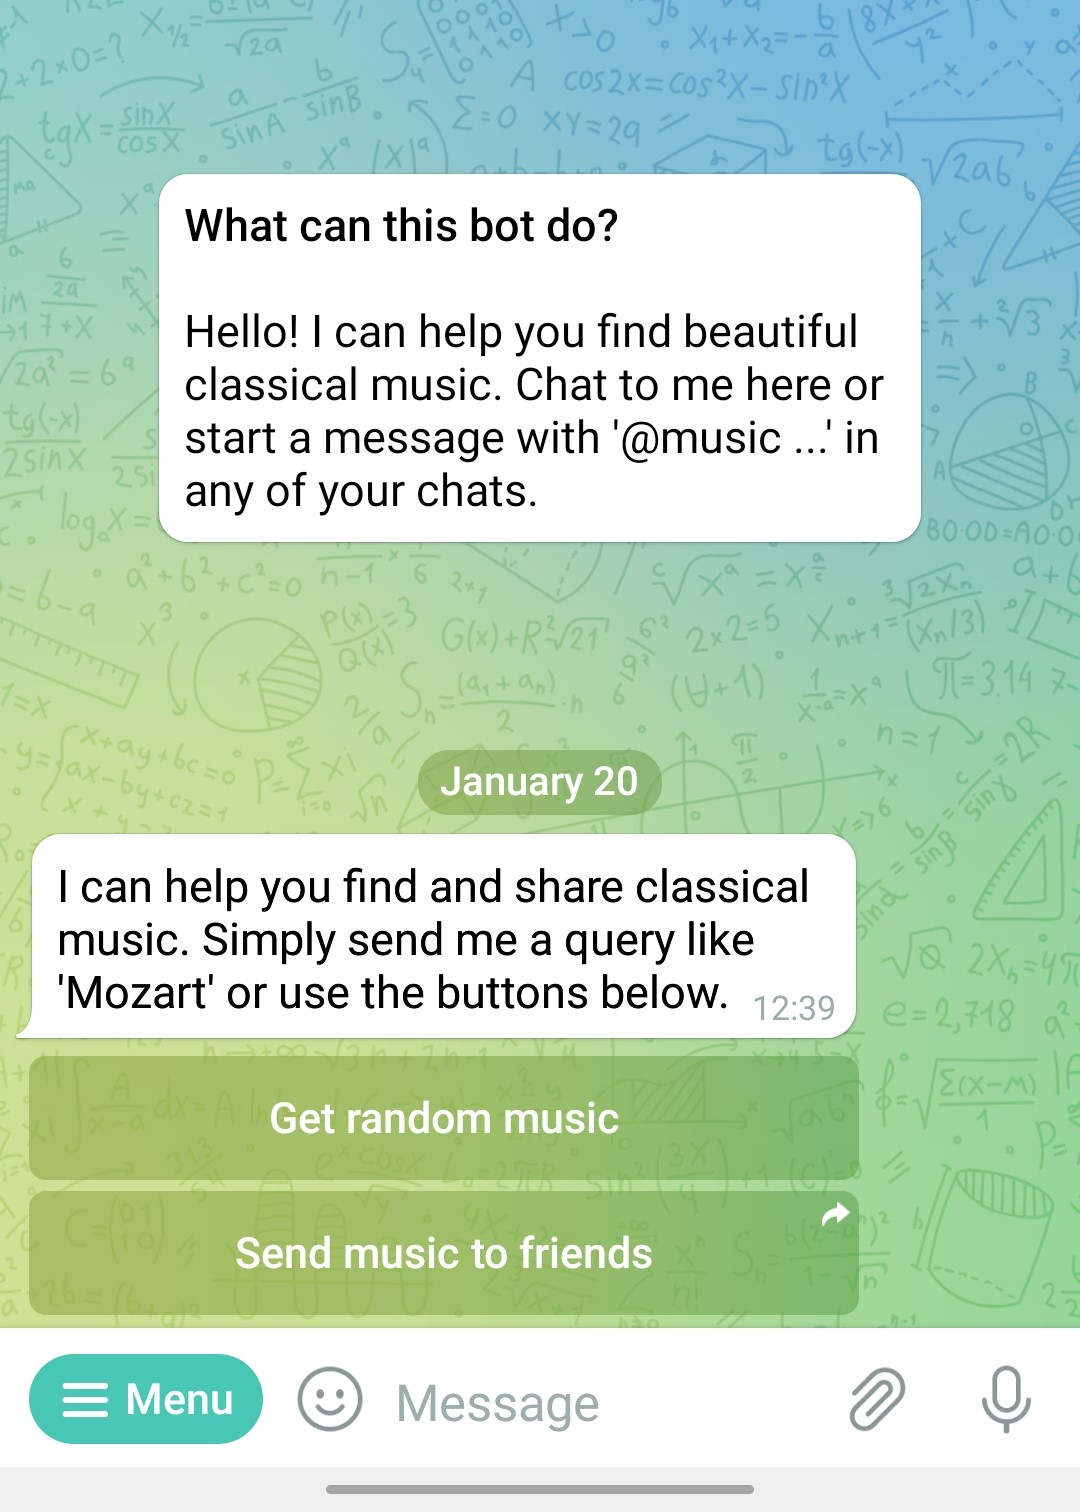
\includegraphics[width=\linewidth]{tastiera_inline.jpg}}
\caption{Tastiera inline}
\label{fig:inline_keyboard}
\end{subfigure}\hfil 
\begin{subfigure}{0.25\textwidth}
\frame{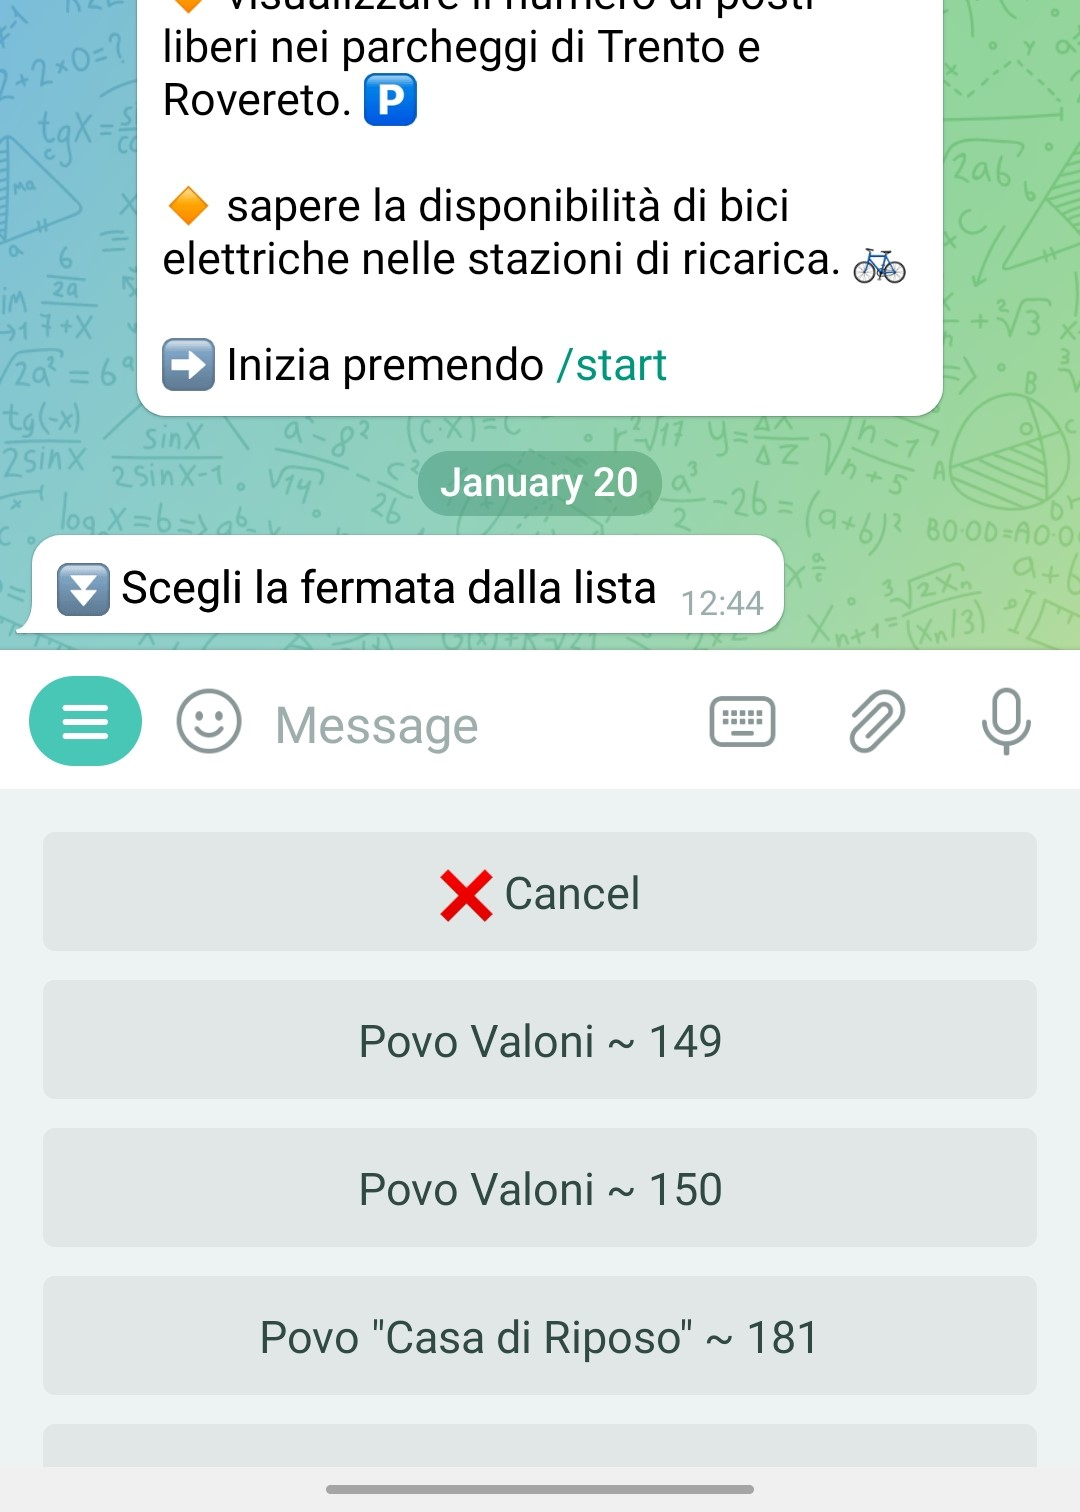
\includegraphics[width=\linewidth]{tastiera_normale.jpg}}
\caption{Tastiera normale}
\label{fig:normal_keyboard}
\end{subfigure}

\caption{
\label{fig:telegram_interactions}Interazioni Telegram bot}
\end{figure}

\pagebreak

\section{Analisi dei requisiti}
\label{sec:requisiti}

Come descritto in precedenza lo scopo principale di questo bot è raccogliere in unico applicativo varie informazioni sui trasporti pubblici della Provincia di Trento. 
In particolare si vuole dare la possibilità agli utenti di:
\begin{itemize}
\item consultare gli orari di autobus urbani e extraurbani;
\item consultare gli orari delle ferrovie Brennero, Valsugana e Trento-Mezzana;
\item visualizzare su una mappa dove si trova un autobus in tempo reale e avere la possibilità di seguirlo durante il suo percorso;
\item visualizzare il ritardo e l'ultima posizione conosciuta dei mezzi;
\item visualizzare il numero di posti liberi nei parcheggi dei comuni di Trento e Rovereto;
\item sapere la disponibilità di bici elettriche presenti nelle stazioni di ricarica;
\item salvare le fermate e linee preferite per una consultazione di orari e ritardi molto più veloce;
\item rimanere informati su eventuali scioperi, variazioni di percorso, fermate sospese.
\end{itemize}

Alcuni requisiti, come l'acquisto dei biglietti e la ricerca dei singoli percorsi, sono stati esclusi. In particolare, il primo per difficoltà nella vendita dei biglietti, data la mancanza di API pubbliche apposite; mentre il secondo, per una scelta personale. 




\section{Progettazione}
\label{sec:progettazione}

Il prodotto, in questo caso il Bot, deve essere progettato intorno alle persone. Quindi, per avere una più chiara visione dei comportamenti, abitudini e bisogni del nostro target di riferimento ho deciso di creare 2 personas e 2 scenari.

I \textit{personas} sono personaggi di fantasia che rappresentano un possibile gruppo di utenti reali. Mentre, gli \textit{scenari} consistono in una ricostruzione dettagliata di una situazione d'utilizzo. 

\subsection{Personas}
\begin{itemize}
\item \textbf{Antonio} è uno studente universitario pendolare di 21 anni, abita a Rovereto e, quindi, utilizza il treno e i bus di linea per andare in università, in biblioteca o in mensa. Ogni mattina, per controllare gli orari e i ritardi del treno regionale e del bus, ha bisogno di consultare più applicazioni. Gli piacerebbe, quindi, avere un unico applicativo per poter controllare tutti le informazioni necessarie.
\item \textbf{Francesca} è una turista di 35 anni, è arrivata in Trentino in treno. Durante la sua permanenza ha deciso di utilizzare solo i mezzi pubblici e le bici elettriche in sharing per raggiungere i vari luoghi di interesse. Ha molta dimestichezza con i dispositivi digitali, la sua esigenza chiave è poter visitare più destinazioni possibili e non perdere tempo inutilmente.  
\end{itemize}

\subsection{Scenari}
\begin{itemize}
\item \textbf{Scenario A}: l'utente è alla fermata dell'autobus e sono già passati 5 minuti dall'orario previsto di arrivo, decide allora di controllare sul bot Telegram il ritardo accumulato. Una volta scoperto che il ritardo previsto eri di ulteriori 15 minuti, decide di andare a bere un caffè. 
\item \textbf{Scenario B}: l'utente vuole prendere una bici elettrica in sharing, una volta arrivato alla stazione di ricarica non ne trova nessuna disponibile. Controlla allora sul bot qual è la stazione più vicina alla sua posizione attuale dove poter trovare una bici. 
\end{itemize}


\subsection{Servizi esterni}

Per fornire dati reali e utili è stato necessario avvalersi di vari servizi esterni. In particolare: 
\begin{itemize}
\item gli orari e le informazioni sulle fermate degli autobus urbani ed extra urbani sono forniti in formato CSV dal sito \textit{opendata} di Trentino Trasporti \cite{opendataTrentinoTrasporti}
\item le informazioni in tempo reale provengono dalle API dell'applicazione \textit{Muoversi in Trentino}
\item gli orari dei treni sono fornite dalle API del servizio \textit{ViaggiaTreno}
\item i dati sui parcheggi e sulle stazioni di ricarica delle biciclette provengono dalle API delle applicazioni mobile \textit{ViaggiaTrento} e \textit{ViaggiaRovereto}.
\end{itemize}

\subsection{Struttura e interfaccia del bot}
Il bot è stato pensato per funzionare sia utilizzando la tastiera inline che i comandi. 
L'interfaccia con cui ci troveremo ad interagire presenterà una serie di pulsanti inline con i quali sarà possibile navigare tra le diverse funzioni. Le informazioni saranno inviate prevalentemente tramite messaggi testuali arricchiti da emoji utili a rende l'esperienza dell'utente più dinamica e comprensibile. 
Un'ulteriore funzionalità sarà la possibilità di osservare su una mappa, in tempo reale, l'ultima posizione rilevata di un autobus e per fare ciò verrà utilizzata la funzione di \textit{live location} fornita da Telegram. 
Le news su eventuali scioperi, variazioni di percorso, fermate sospese, invece, verranno inviate automaticamente dal bot su un canale Telegram dedicato. 

\subsection{Database}
Il bot avrà bisogno di un database in cloud per gestire le preferenze degli utenti, come fermate e linee preferite, e le sessioni di questi. In particolare, si dovranno gestire le sessioni in quanto i messaggi di Telegram sono inviati in maniera indipendente uno dall'altro. Risulta quindi necessario un meccanismo per gestire scenari complessi in cui un'azione dipende da una precedente. 

\pagebreak

\section{Tecnologie utilizzate}
\label{sec:tecnologie}

Le tecnologie utilizzate per l'implementazione di questo bot saranno descritte brevemente di seguito. 

\subsection{Node.js}

\begin{wrapfigure}{r}{0.33\textwidth}
\centering

\includegraphics[width=2.5cm]{nodejs-logo.png}
\caption{Logo NodeJS}
\end{wrapfigure}

\textit{Node.js} è un runtime JavaScript guidato da eventi asincroni ed è progettato per creare applicazioni di rete scalabili. Alcuni dei principali vantaggi di Nodejs sono le ottime performance, un processo di sviluppo facilitato e un'ottima scalabilità. Inoltre, utilizzandolo si ha accesso al più grande ecosistema di librerie open source al mondo: \textit{Node Package Manager} (NPM).

\subsection{telegraf.js}

\begin{wrapfigure}{r}{0.33\textwidth}
\centering

\includegraphics[width=2.5cm]{telegraf-logo.png}
\caption{Logo telegraf.js}
\end{wrapfigure}

Telegram per creare i bot mette a disposizione della API HTTPS. Lo sviluppatore può scegliere se utilizzarle come sono fornite oppure avvalersi di una delle tante librerie esistenti per i principali linguaggi di programmazione. Esse sono ormai il metodo suggerito, poiché semplificano molto lo sviluppo e offrono la possibilità di aggiungere funzionalità extra. Per Node.js esistono varie librerie, io ho scelto di utilizzare \textit{telegraf.js} perché ritengo sia la più completa e molto supportata dalla comunità. Essa è anche estensibile attraverso ulteriori librerie che danno la possibilità di introdurre altre feature.

\subsection{MongoDB}

\begin{wrapfigure}{r}{0.33\textwidth}
\centering

\includegraphics[width=3cm]{mongodb-logo.png}
\caption{Logo MongoDB}
\end{wrapfigure}

\textit{MongoDB} è un DBMS non relazionale, orientato ai documenti. Classificato come un database di tipo NoSQL, MongoDB si allontana dalla struttura tradizionale basata su tabelle dei database relazionali in favore di documenti in stile JSON con schema dinamico (MongoDB chiama il formato BSON), rendendo l'integrazione di dati di alcuni tipi di applicazioni più facile e veloce \cite{Mongodb}. Le principali caratteristiche sono che la replicazione di un database (\textit{Replica Set}) può avvenire in modo molto semplice, e che garantisce la scalabilità automatica, ossia la possibilità di distribuire (Sharding) le collezioni in cluster di nodi, in modo da supportare grandi quantità di dati senza influire pesantemente sulle performance.

\subsection{Redis}

\begin{wrapfigure}{r}{0.33\textwidth}
\centering

\includegraphics[width=3cm]{redis-logo.png}
\caption{Logo Redis}
\end{wrapfigure}

\textit{Redis}, acronimo di Remote Dictionary Server, è un archivio dati veloce, open source, in memoria e di tipo chiave-valore. Esso può essere utilizzato come database, sistema di caching o come broker di messaggi. Redis offre tempi di risposta inferiori al millisecondo ed è per questo una scelta popolare per caching, gestione della sessione, giochi, classifiche, analisi dei dati in tempo reale, geospazialità, ride-hailing, chat/messaggistica, streaming multimediale e app pub/sub. \cite{Redis}

\pagebreak

\section{Implementazione}
\label{sec:implementazione}

Per l'implementazione di questo bot ho scelto di utilizzare \textit{NodeJs} utilizzando \textit{Typescript} come linguaggio di programmazione. \textit{Typescript} mi ha permesso di utilizzare la programmazione ad oggetti e di tipizzare le risposte ottenute dalle API, rendendo il codice molto più strutturato e solido.  Durante lo sviluppo mi sono avvalso di alcune librerie presenti su NPM tra cui \textit{telegraf.js} per l'implementazione delle chiamate alle API di Telegram, \textit{Axios} per poter chiamare in modo agevole le API dei servizi esterni descritti in precedenza e \textit{mongoose} per potermi interfacciare con il database MongoDB.

Per gestire le sessioni ho utilizzato un estensione della libreria telegraf.js che permette di salvare e gestire la sessione degli utenti nel database MongoDB, questo ha semplificato la gestione dei flussi più complessi che richiedono all'utente di inserire più informazioni. 

\subsection{Architettura}
\label{sec:architettura}

L'architettura del bot Telegram è rappresentata in figura \ref{fig:architettura_bot}.

\begin{figure}[h]
\centering
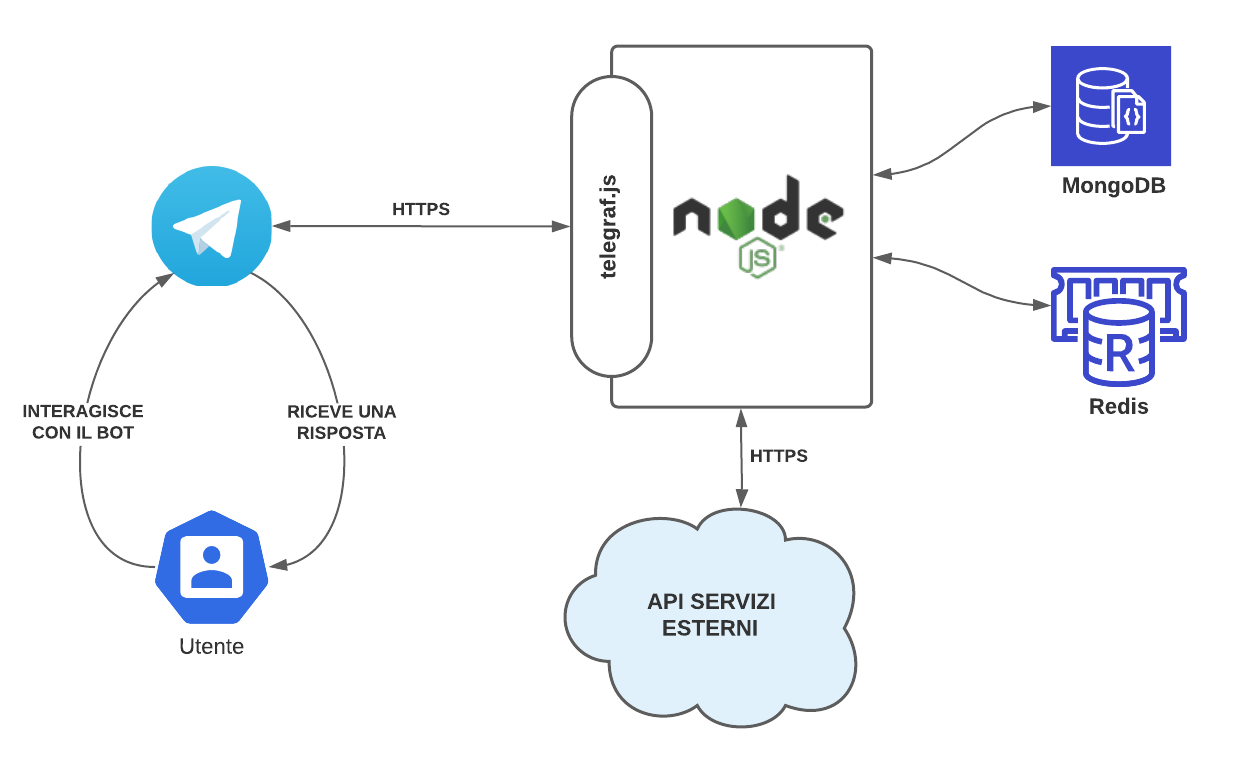
\includegraphics[width=0.8\textwidth]{architettura-bot.png}
\caption{Architettura del bot}
\label{fig:architettura_bot}
\end{figure}

Come si può osservare dalla figura, quando un utente invia una richiesta (messaggio, comando, posizione, ...) dall'applicazione Telegram, le informazioni vengono processate dai server di quest'ultima e sono rese disponibili attraverso le Bot API. La libreria \textit{telegraf.js} si occupa, quindi, dell'interazione con queste API rendendole disponibili al backend \textit{Nodejs}. Il backend si occupa di gestire le informazioni ricevute e restituisce all'utente una risposta adeguata. Per fare ciò potrà avvalersi dei servizi esterni e dei database. Il database MongoDB è utilizzato sia per mantenere le sessioni e le preferenze degli utenti che per memorizzare gli orari degli autobus mentre Redis è utilizzato come sistema di caching. Maggiori dettagli sullo scopo e l'utilizzo dei database sono adeguatamente forniti nel paragrafo \ref{sec:problemi}.

\pagebreak

\noindent Di seguito un esempio concreto: 
\begin{enumerate} 
\item l'utente invia al bot, attraverso un comando, una richiesta di orario per la fermata Piazza Dante; 
\item la richiesta viene processata dai server di Telegram, e resa disponibile attraverso una Bot API;
\item il backend di \textit{Nodejs}, attraverso l'interfaccia \textit{telegraf.js}, riceve l'informazione;
\item il backend contatta il database per estrarre gli orari e l'API esterna per l'informazione in tempo reale;
\item una volta raccolte tutte le informazioni, \textit{Nodejs} formatterà un messaggio di risposta; 
\item questo verrà inviato, attraverso le Bot API, a Telegram; 
\item l'utente riceverà la risposta sul proprio dispositivo. 
\end{enumerate}

\noindent In figura \ref{fig:bpmn_autobus_flow} è rappresentato, attraverso l'utilizzo di un \textit{Business Process Modeling Notation} (BPMN), il processo di richiesta e visualizzazione degli orari di una fermata autobus urbana. Il diagramma è stato semplificato in modo da raffigurare solo il flusso principale e tralasciando la gestione dei casi limite.

\begin{figure}[h]
\centering
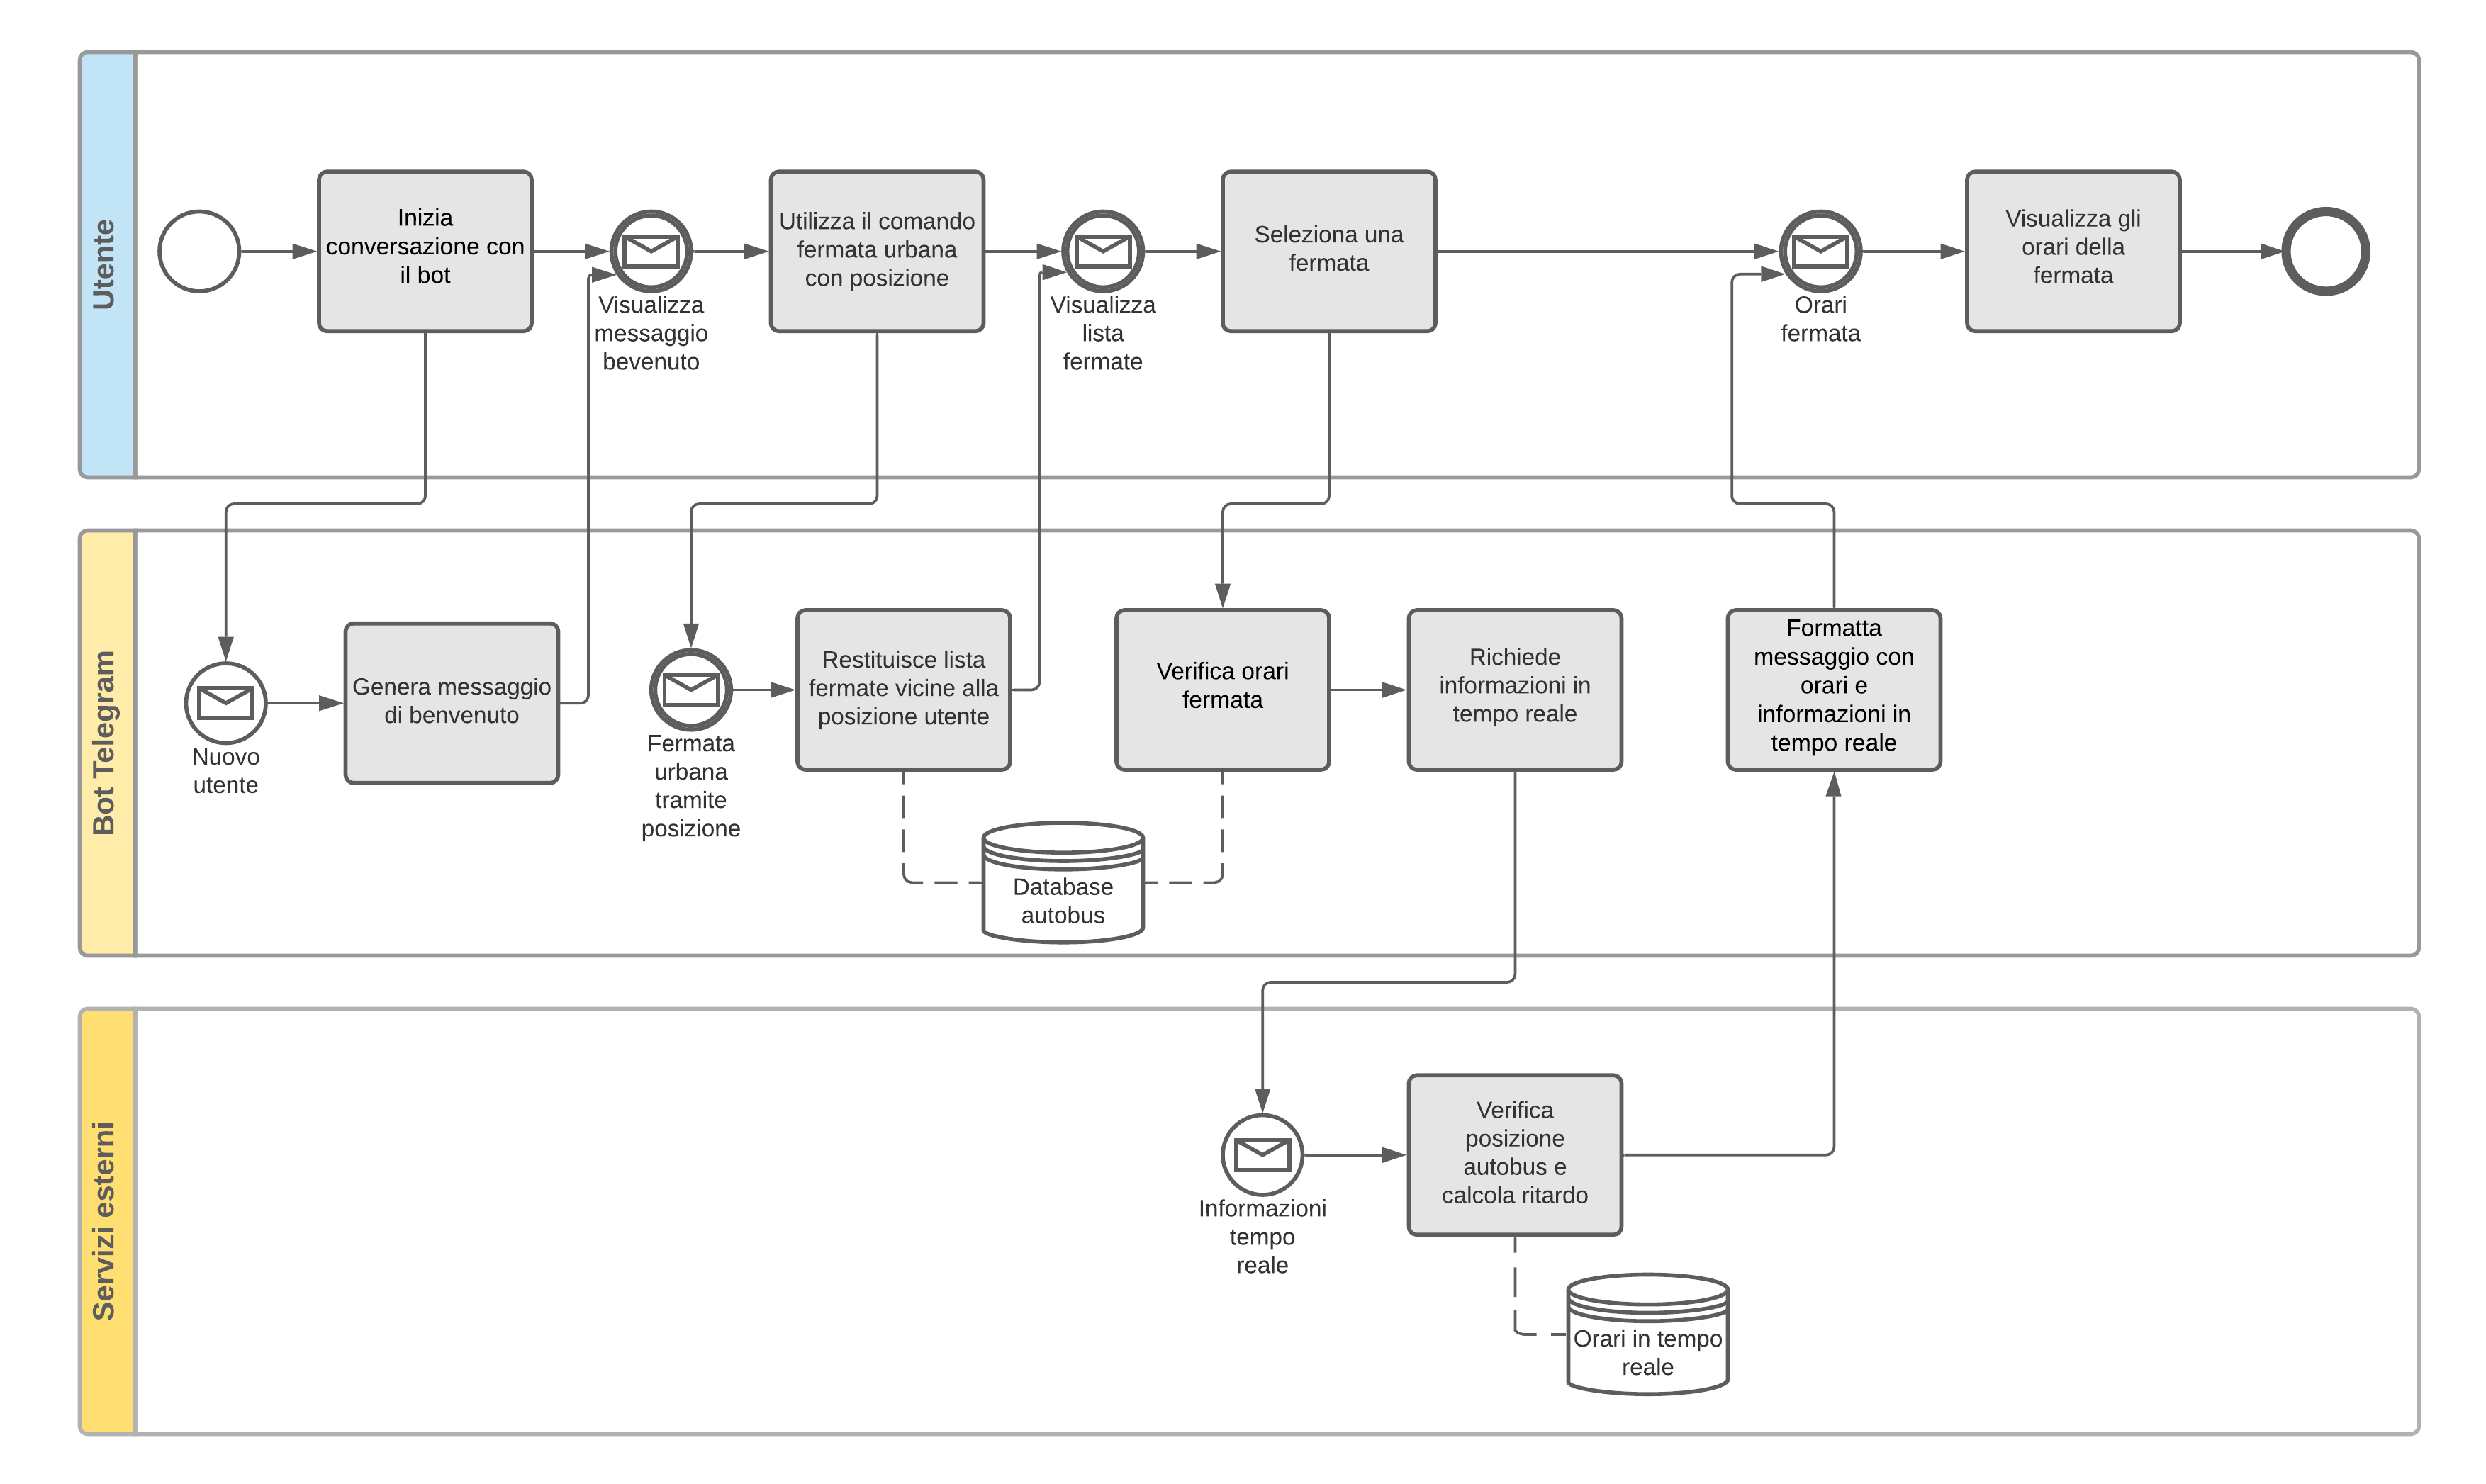
\includegraphics[width=\textwidth]{bot-bpmn-autobus-flow.png}
\caption{BPMN flusso richiesta orari fermata autobus}
\label{fig:bpmn_autobus_flow}
\end{figure}

\newpage
\newpage

\subsection{Continuous deployment e ambiente di produzione}
\label{sec:produzione}

Per l'hosting dell'applicativo \textit{NodeJS} ho deciso di utilizzare una VPS Ubuntu fornita dal provider tedesco \textit{Hetzner}. Sulla macchina virtuale ho poi installato, un process manager, \textit{PM2}. Esso permette di semplificare alcuni compiti da amministratore di sistema, come riavviare l'applicativo in caso di crash, aggiornare il sistema senza avere momenti di inattività, mantenere e monitorare i log e implementa anche un sistema di load-balancing. Dato che il codice del bot è salvato su una repository Github, ho potuto utilizzare le \textit{Github Actions} per implementare un sistema di \textit{continuous deployment}. Ad ogni push sulla master branch viene attivato il flusso di pubblicazione che transpila il codice da Typescript a Javascript e copia quest'ultimo nella VPS ubuntu utilizzando il protocollo SSH. Grazie alla funzionalità di PM2, che permette di riavviare il programma in caso di cambiamenti nel codice, dopo pochi secondi la nuova versione è pubblicata e disponibile agli utenti. Il database Redis è installato e presente all'interno della VPS mentre il database MongoDB è esterno in un hosting \textit{Google Cloud} dedicato.

\begin{figure}[h]
\centering
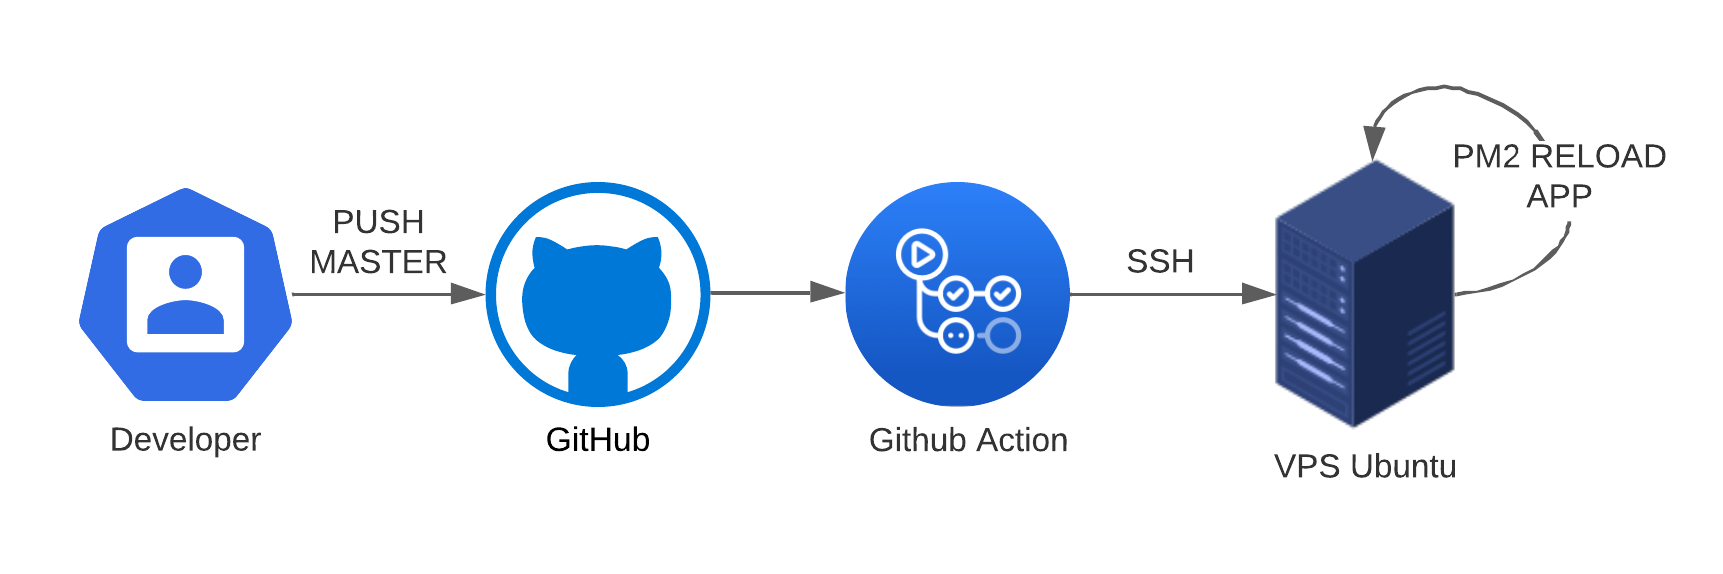
\includegraphics[width=0.80\textwidth]{continuous-deployment.png}
\caption{Flusso di distribuzione continua}
\label{fig:continuous_deployment}
\end{figure}

\section{Analisi dei principali problemi}
\label{sec:problemi}

Durante lo sviluppo di questo Bot ho incontrato alcuni problemi. La difficoltà maggiore riguarda la gestione delle API esterne che, a volte, non risultano disponibili. Per mitigare questo problema ho, in primo luogo, inserito dei messaggi di errore che informavano l'utente della presenza di un problema riscontrato non dipendente dal Bot, ma dai servizi esterni. 
In particolare, le API che presentano maggiormente questo problema sono quelle che restituiscono le informazioni in tempo reale degli autobus. In un primo momento, queste API venivano utilizzate anche per conoscere gli orari, ma data la frequente assenza di questi dati, ho deciso di aggiungere al database \textit{MongoDB} una copia di tutte le informazioni sulle fermate e sulle linee. Questo permette di chiamare l'API solo per i dati in tempo reale, permettendo comunque all'utente di ricevere gli orari con l'avviso della temporanea mancanza dei ritardi e della posizione. 
Dopo l'introduzione di questa soluzione, ho notato che le risposte all'utente, vista la necessità del doppio passaggio, richiedevano dei tempi di caricamento maggiori. Per ovviare a questo problema, ho introdotto un sistema di \textit{caching} del database \textit{MongoDB} utilizzando \textit{Redis} e ho implementato anche un sistema di \textit{caching} per le risposte ottenute dall'API esterne. Ciò ha permesso di migliorare l'esperienza dell'utente, riducendo sensibilmente i tempi di risposta. 

\newpage

\section{Funzionamento ed interfaccia utente}
\label{sec:funzionamento}

La sezione seguente è dedicata all'analisi, attraverso la presentazione dell'interfaccia utente, del funzionamento generale e delle caratteristiche del bot. La descrizione è accompagnata da alcune schermate tratte dall'applicazione mobile di Telegram in modo da rendere più chiaro di cosa si sta parlando.

\subsection{Menu iniziale}

\begin{wrapfigure}{r}{0.45\textwidth}
\centering
\frame{
\includegraphics[scale=0.14]{bot-menu-iniziale.jpg}}
\caption{Menu iniziale}
\label{fig:bot-menu-iniziale}
\end{wrapfigure}

Una volta aperta la chat privata con il bot Telegram, \textit{@TrentinoInBusBot}, ci si trova davanti ad un messaggio di benvenuto che descrive brevemente le funzionalità del bot. Per iniziare è necessario inviare il comando \textit{/start}. L'utente riceverà a questo punto un messaggio con una \textit{tastiera inline}. Tramite quest'ultima, come si può notare nella figura \ref{fig:bot-menu-iniziale}, si è voluto creare un menu iniziale, che raggruppa in categorie le funzionalità principali, e da la possibilità di navigare ed utilizzare il bot in maniera semplice.

Come si vedrà anche successivamente, ogni messaggio inviato dal bot avrà sempre una \textit{tastiera inline} allegata che permette di ritornare al menu principale o di compiere diverse azioni a seconda della funzionalità che stiamo utilizzando. L'utilizzo di queste tastiere permette al bot di essere molto più simile ad un applicazione mobile tradizionale, di guidare l'utente e di essere intuitivo anche per utenti al primo utilizzo. Per rendere l'interfaccia più accattivante e accessibile sono state inserite delle \textit{emoji}.

In alternativa al menu principale, il bot mette a disposizione anche dei comandi scorciatoia che permettono di accedere alle funzionalità più velocemente. Ad esempio, un utente invece che premere sul pulsante \textit{Bici}, visibile in figura \ref{fig:bot-menu-iniziale}, potrebbe semplicemente utilizzare il comando \textit{/bici} e otterrebbe lo stesso risultato.

\subsection{Funzionalità autobus}

\begin{figure}[htb]
    \centering 
\begin{subfigure}{0.20\textwidth}
\frame{
\includegraphics[width=\linewidth]{bot-selezione-autobus.jpg}}
\caption{Selezione ricerca}
\label{fig:bot-selezione-autobus}
\end{subfigure}\hfil
\begin{subfigure}{0.20\textwidth}
\frame{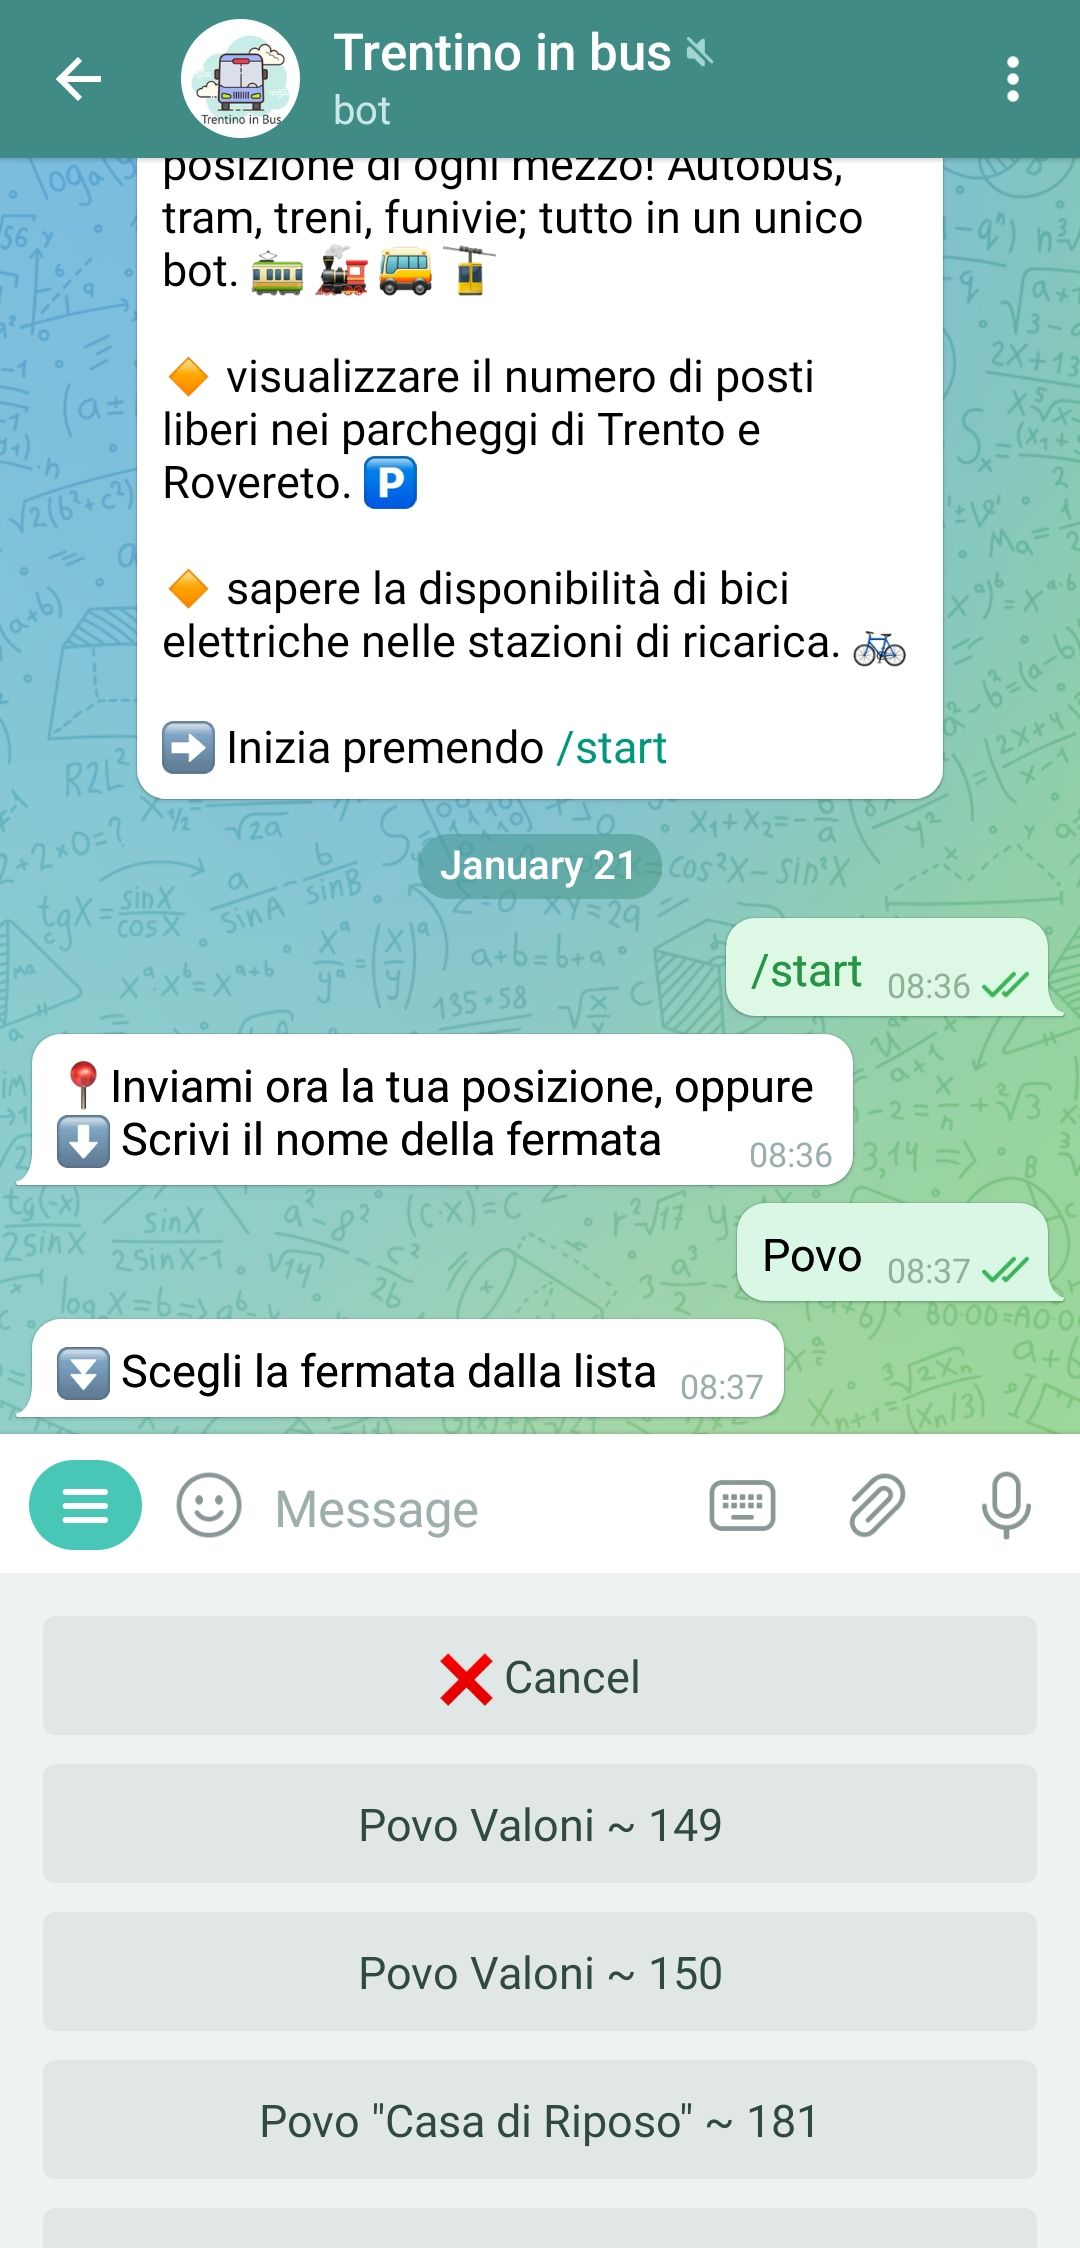
\includegraphics[width=\linewidth]{bot-selezione-fermata.jpg}}
\caption{Ricerca fermata}
\label{fig:bot-selezione-fermata}
\end{subfigure}\hfil 
\begin{subfigure}{0.20\textwidth}
\frame{
\includegraphics[width=\linewidth]{bot-orario-fermata.jpg}}
\caption{Orario fermata}
\label{fig:bot-orario-fermata}
\end{subfigure}\hfil 
\begin{subfigure}{0.20\textwidth}
\frame{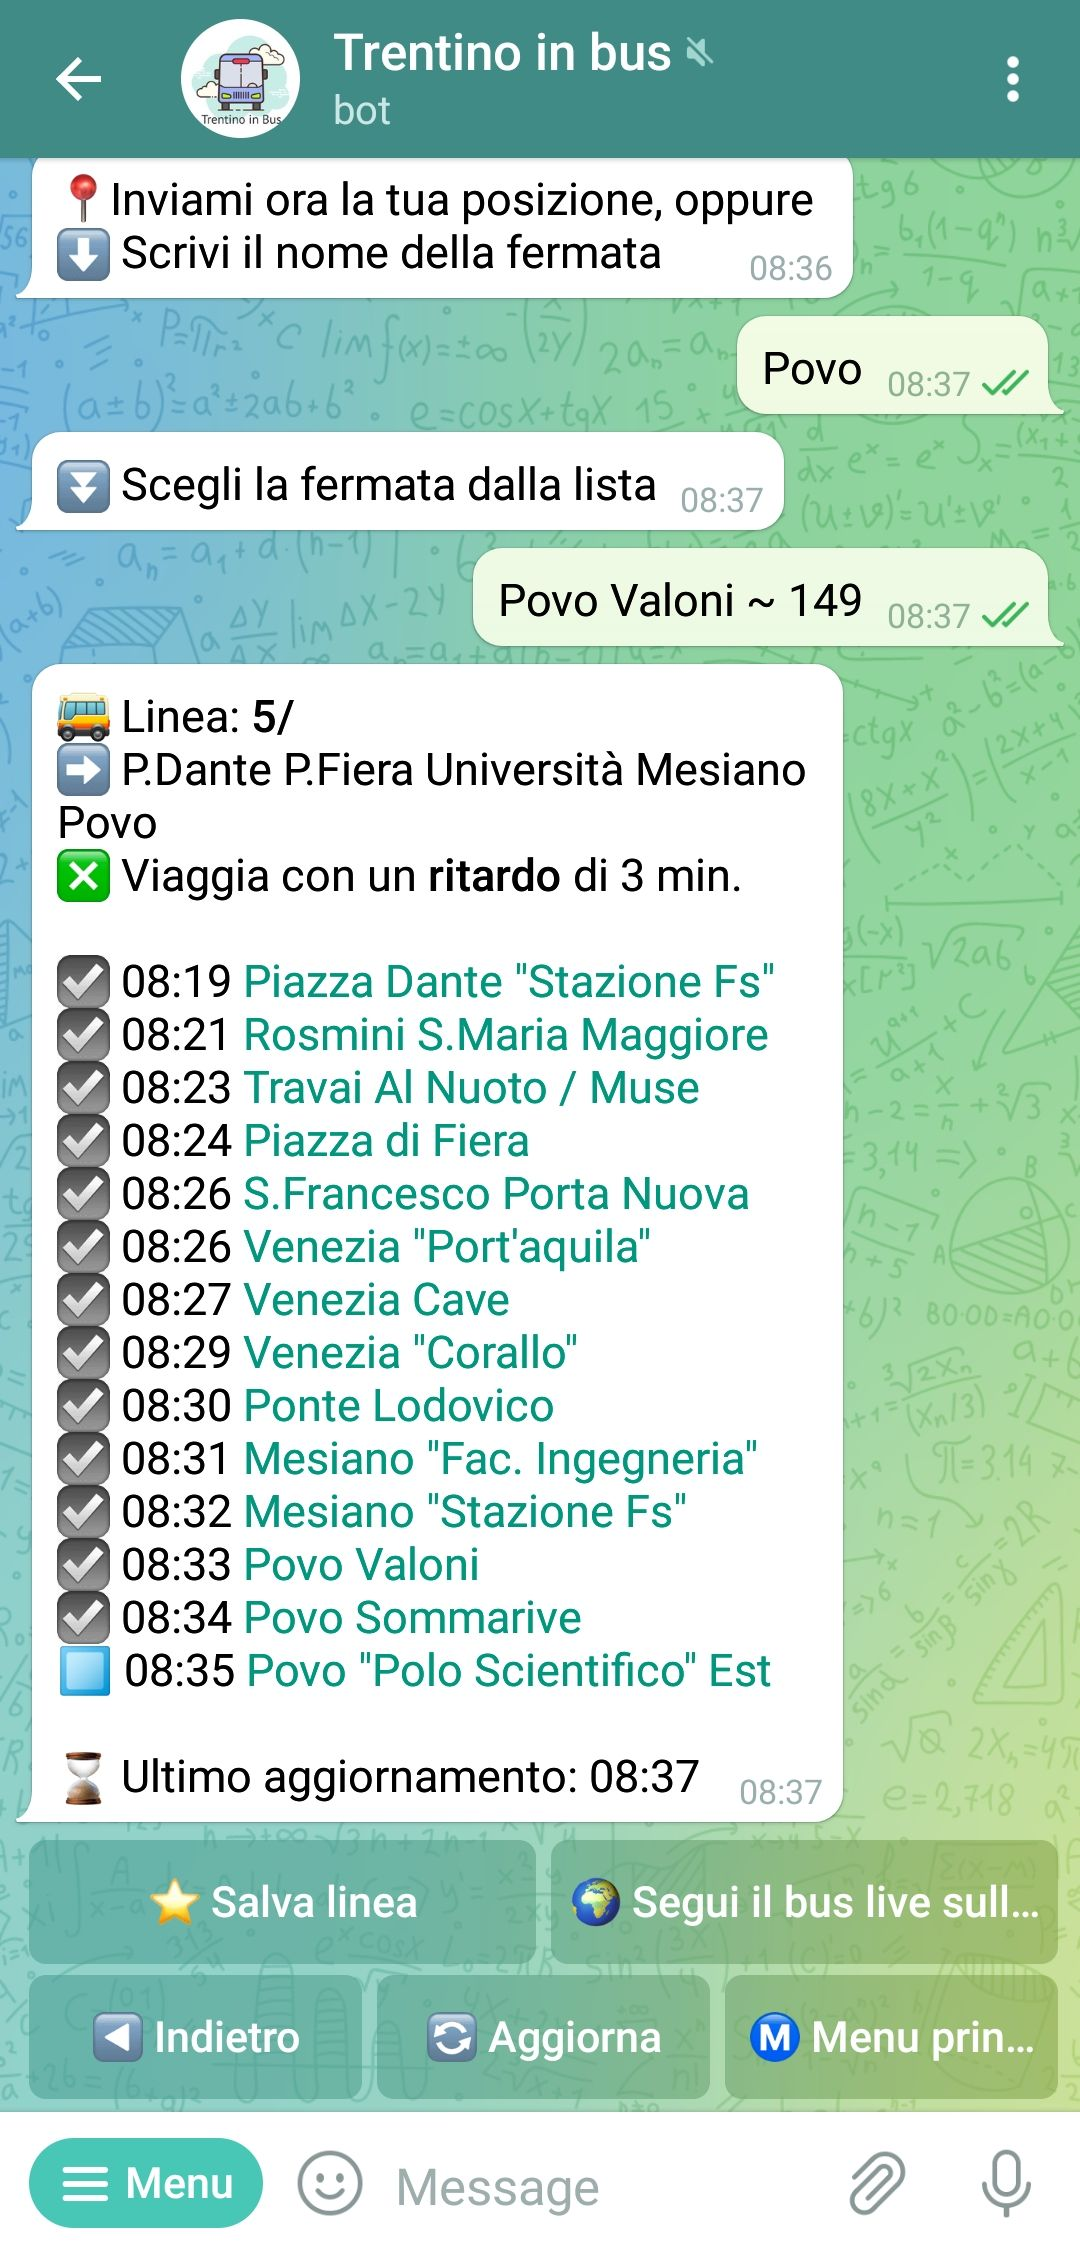
\includegraphics[width=\linewidth]{bot-orari-linea.jpg}}
\caption{Dettaglio linea}
\label{fig:bot-orari-linea}
\end{subfigure}
\caption{
\label{fig:autobus_interfaccia} Interfaccia funzionalità autobus}
\end{figure}

\begin{wrapfigure}{r}{0.33\textwidth}
\centering
\frame{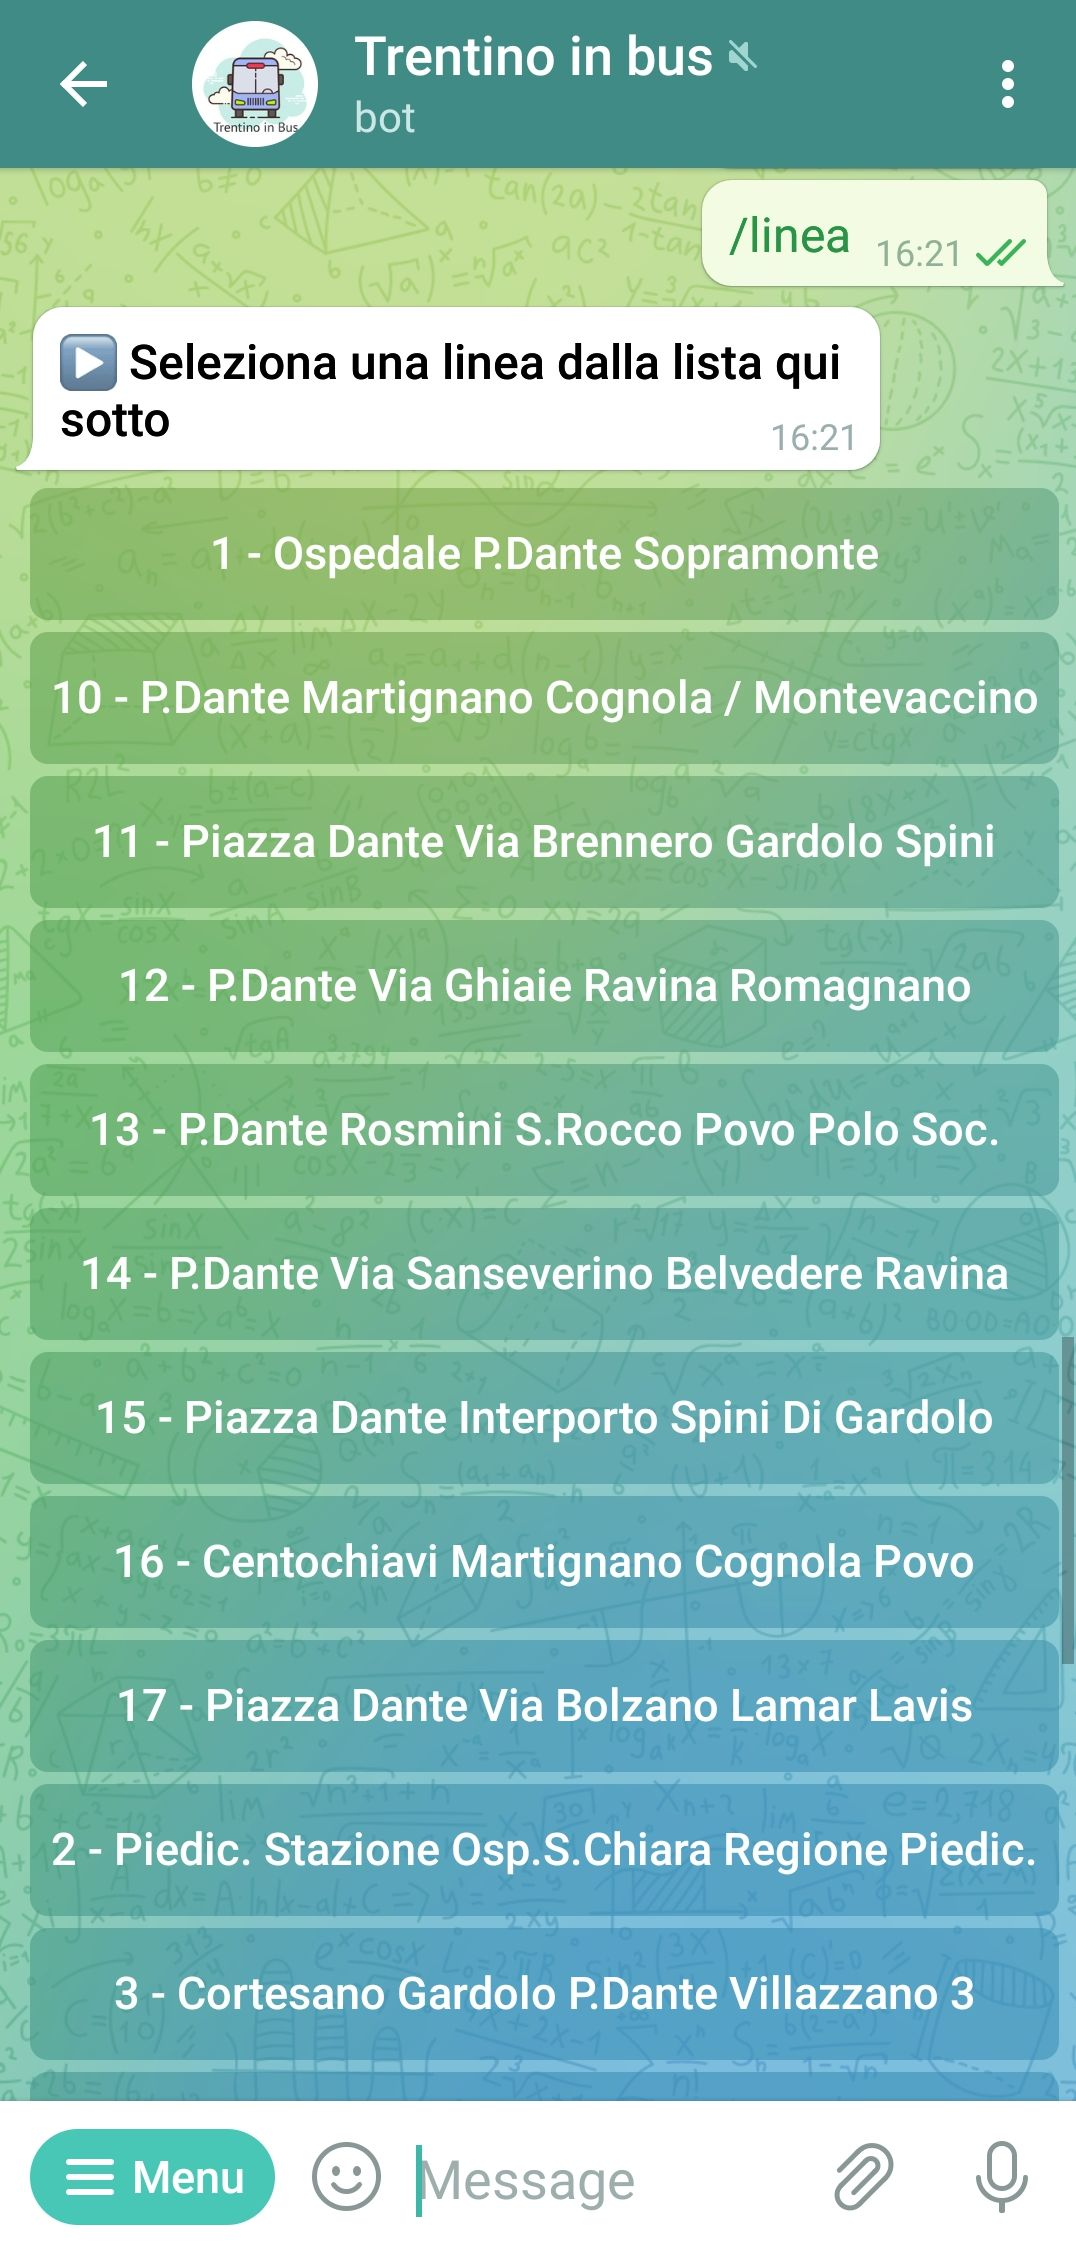
\includegraphics[scale=0.10]{bot-lista-linee.jpg}}
\caption{Lista linee}
\label{fig:bot-lista-linee}
\end{wrapfigure}

Nella figura \ref{fig:autobus_interfaccia} è descritto il funzionamento della funzionalità autobus, in particolare della ricerca degli orari di una fermata. All'utente, una volta premuto il pulsante \textit{Autobus} del menu principale verrà chiesto se intende ricercare una fermata oppure una linea. Premendo sul pulsante \textit{fermata} dovrà poi scrivere il nome della fermata che sta ricercando oppure inviare la propria posizione, a questo punto, a seconda della scelta fatta in precedenza, il bot restituirà una lista di fermate con il nome simile o vicine alla posizione inviata. Dopo aver scelto la fermata di suo interesse, l'utente potrà visualizzare gli autobus in arrivo. Come si nota nella figura \ref{fig:autobus_interfaccia}\subref{fig:bot-orario-fermata} è possibile visualizzare il dettaglio di un solo autobus per volta e, utilizzando i pulsanti \textit{precedente} e \textit{successivo}, è possibile navigare tra gli arrivi. Nel messaggio di dettaglio è presente la linea, il capolinea, l'orario di partenza, l'eventuale ritardo e l'ultima posizione rilevata dell'autobus. Le informazioni in tempo reale si possono aggiornare utilizzando il bottone \textit{Aggiorna}, mentre il bottone \textit{Salva} permette all'utente di salvare la fermata nei propri preferiti. Con il bottone \textit{Fermate} si visualizzerà il messaggio visibile in figura \ref{fig:autobus_interfaccia}\subref{fig:bot-orari-linea}. Quest'ultimo fornisce il dettaglio dell'autobus mostrandone tutte le fermate con il relativo orario di arrivo. Anche qui si ha la possibilità di aggiungere la linea ai preferiti ed è inoltre possibile visualizzare la posizione del bus in tempo reale sulla mappa (funzionalità descritta nel paragrafo \ref{sec:altre_funzionalita}).

Nel caso in cui l'utente scegliesse di ricercare una linea invece che una fermata, il bot proporrà una lista di linee (figura \ref{fig:bot-lista-linee}). L'utente, dopo averne selezionata una, si troverà di fronte un messaggio simile a quello presentato in figura \ref{fig:autobus_interfaccia}\subref{fig:bot-orari-linea} con l'aggiunta, anche in questo caso, dei bottoni \textit{precedente} e \textit{successivo} per navigare tra gli orari.

\subsection{Funzionalità ferrovie}

\begin{wrapfigure}{r}{0.55\textwidth}
    \centering 
\begin{subfigure}{0.23\textwidth}
\centering
\frame{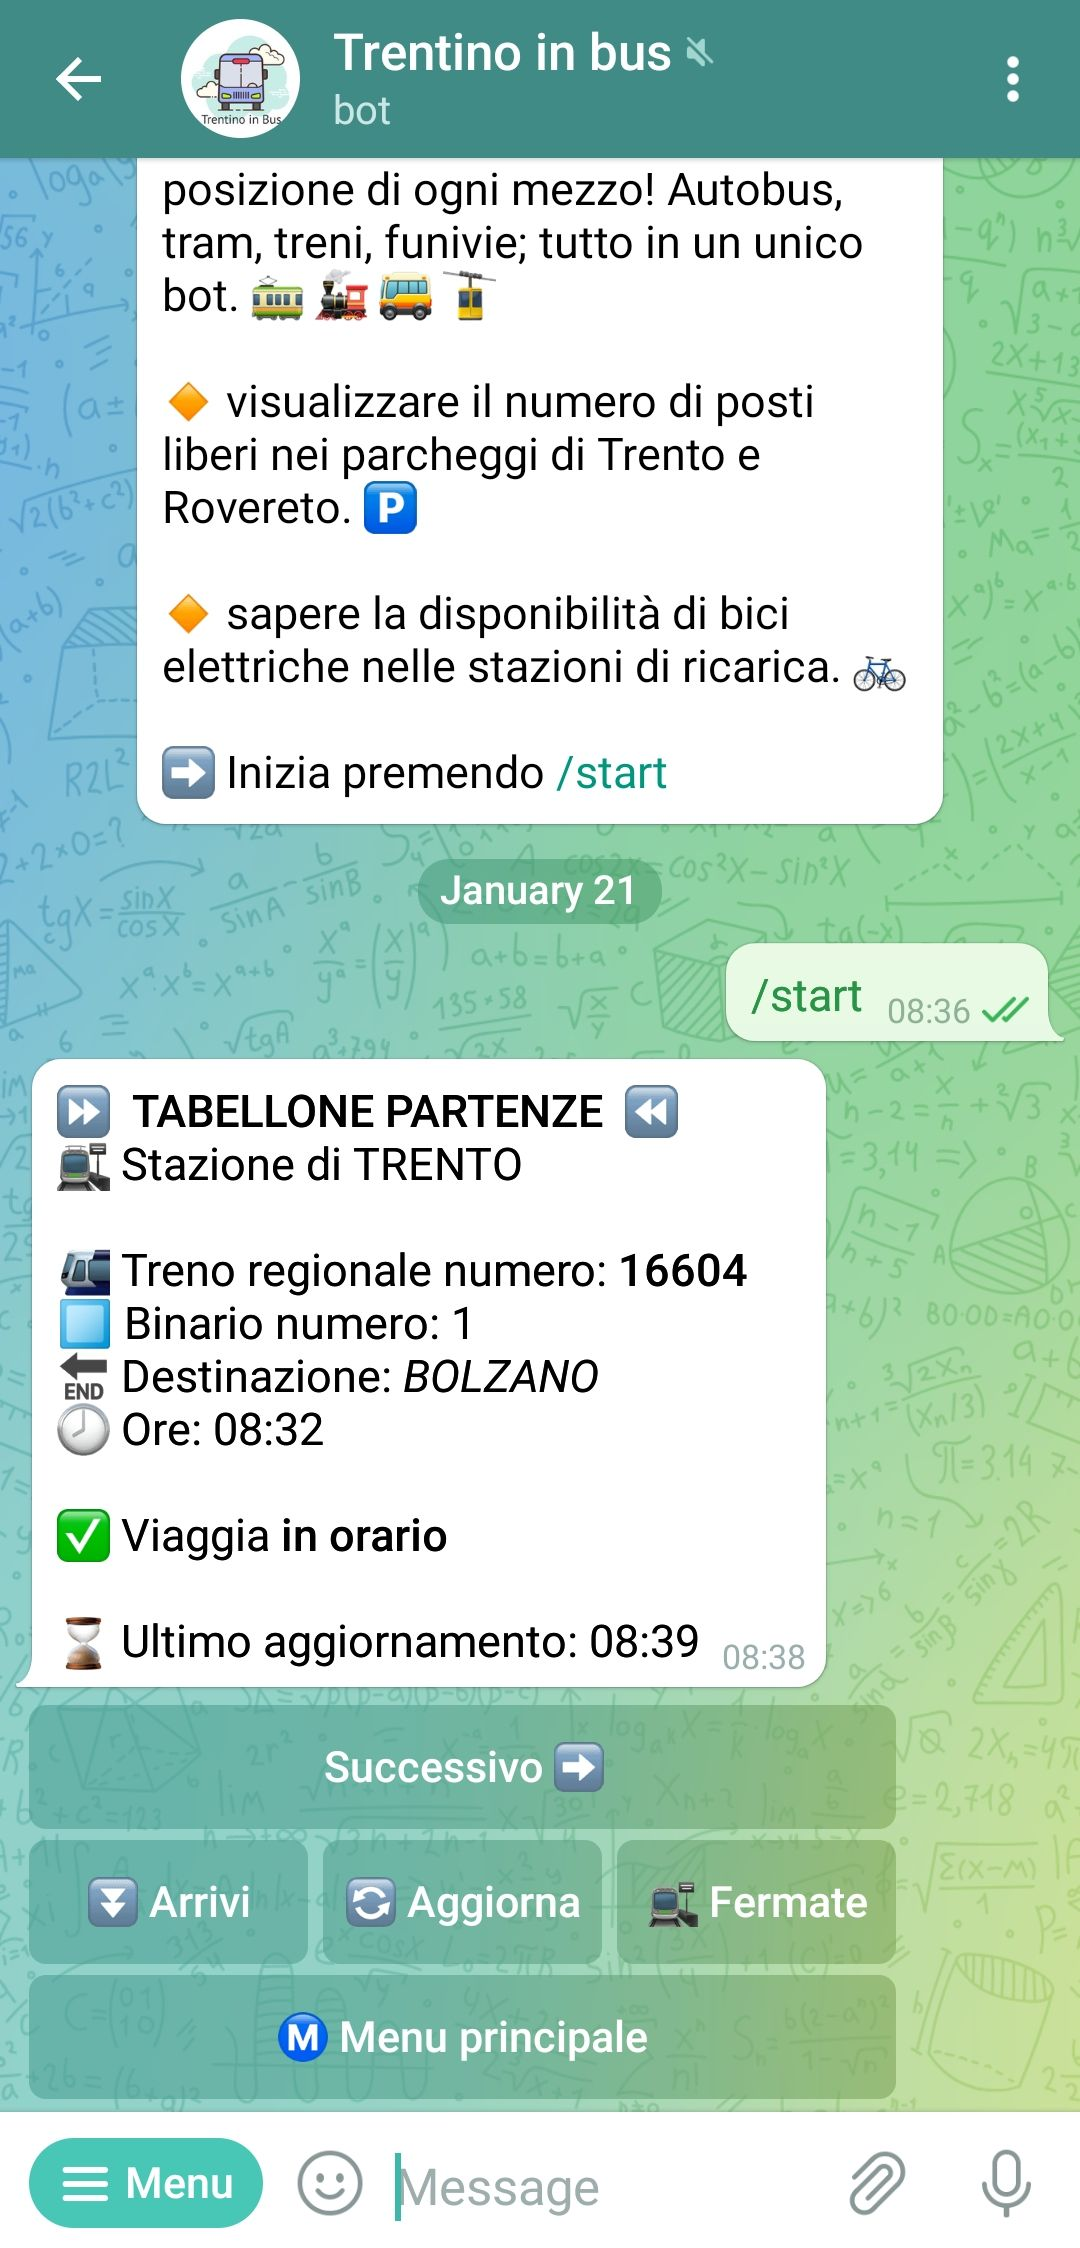
\includegraphics[scale=0.1]{bot-partenze-treno.jpg}}
\caption{Partenze stazione}
\label{fig:bot-partenze-treno}
\end{subfigure}\hfil
\begin{subfigure}{0.23\textwidth}
\centering
\frame{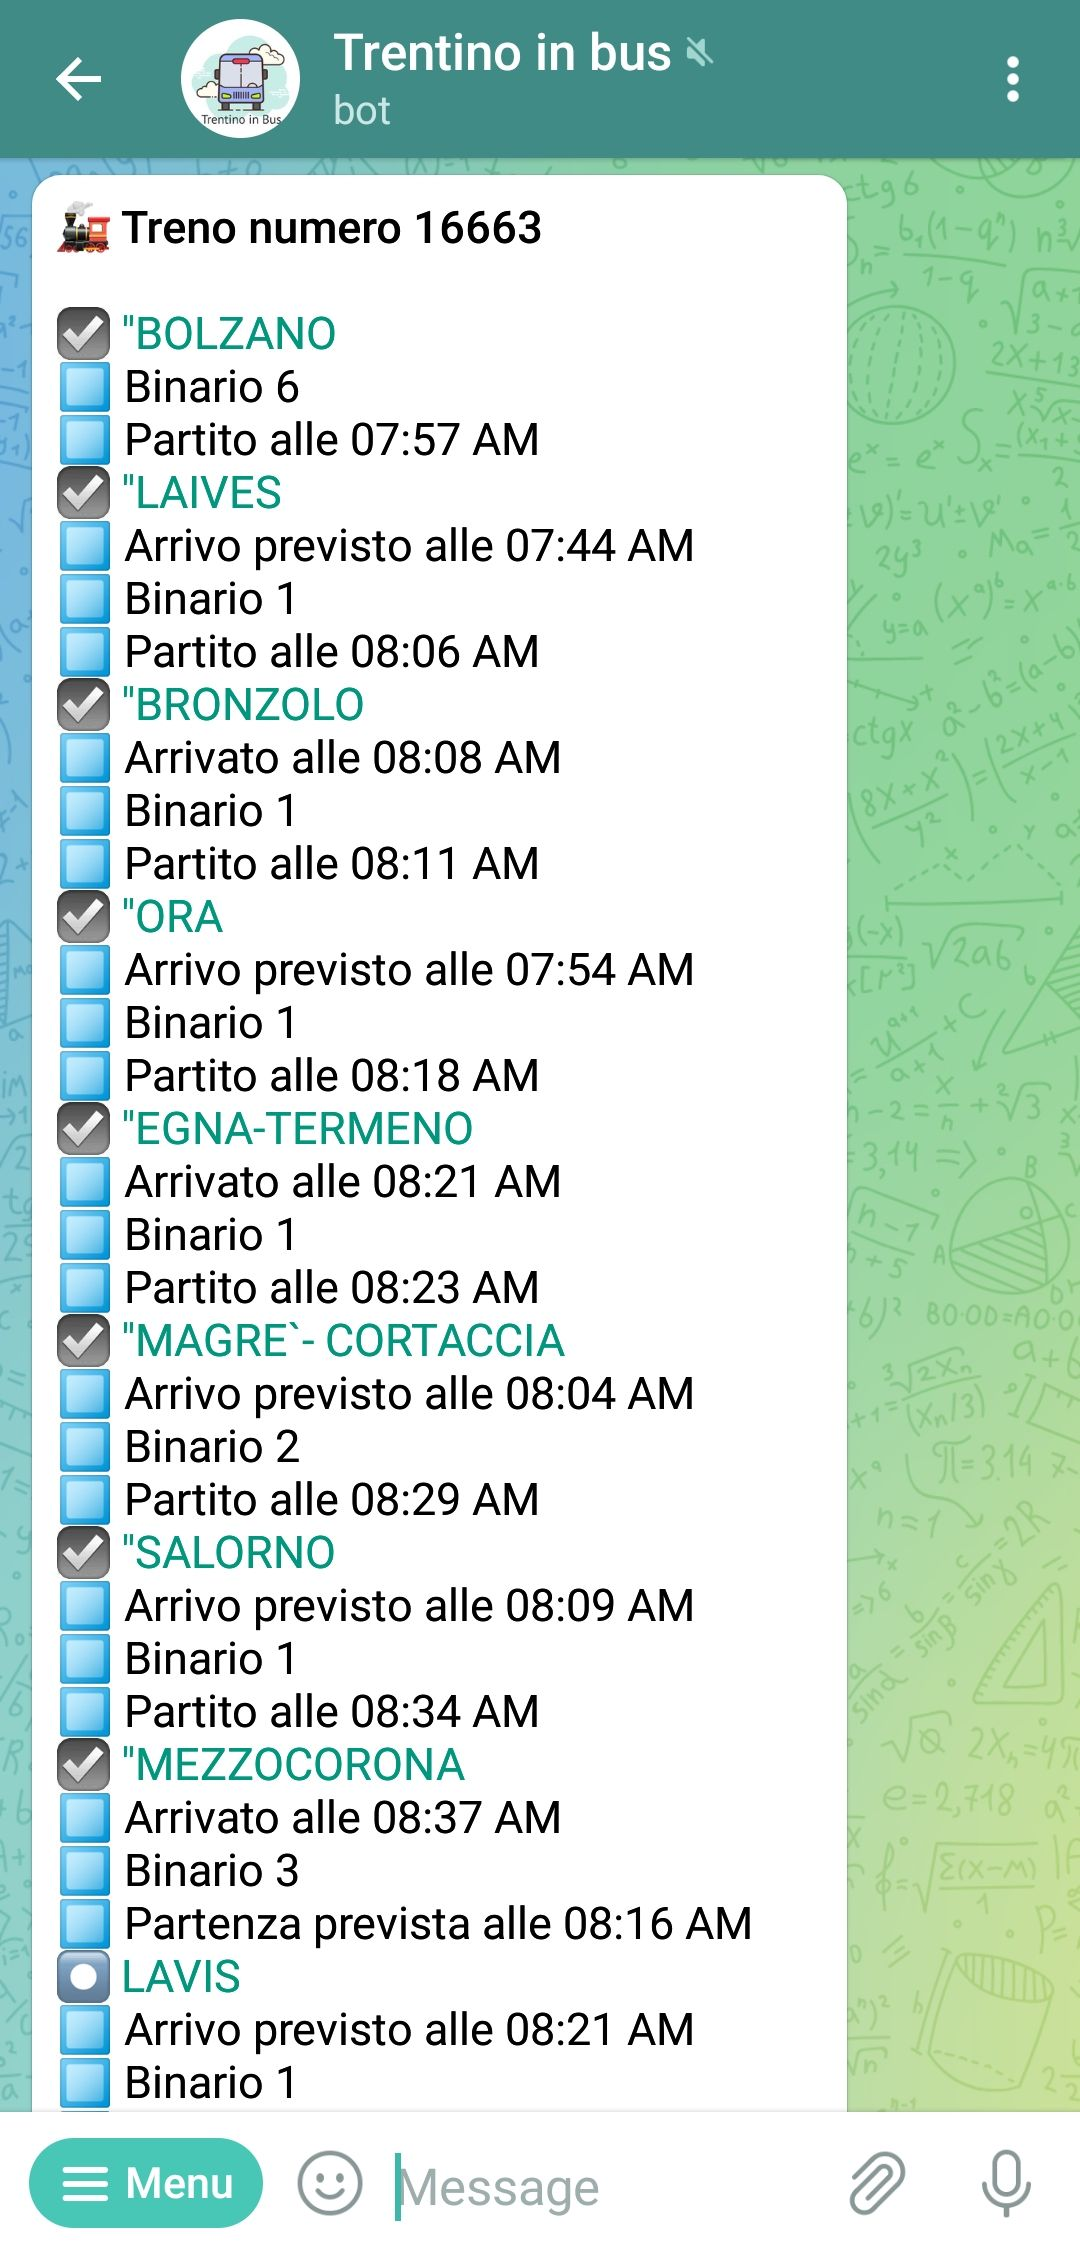
\includegraphics[scale=0.1]{bot-fermate-treno.jpg}}
\caption{Orari fermate}
\label{fig:bot-fermate-treno}
\end{subfigure}
\caption{
\label{fig:treni_interfaccia}Interfaccia funzionalità treni}
\end{wrapfigure}

L'interfaccia della funzionalità ferrovie, esposta in figura \ref{fig:treni_interfaccia}, è molto simile alla funzionalità autobus, ma presenta alcune differenze. Una volta premuto sul bottone \textit{Ferrovie} del menu principale, l'utente dovrà scegliere la ferrovia da visualizzare tra Valsugana, Brennero e Trento-Mezzana. 

Nel caso delle ferrovie gestite da Trenitalia (Valsugana e Brennero) l'utente dovrà scegliere la fermata di suo interesse da una lista e successivamente potrà visualizzarne le partenze e gli arrivi con un messaggio somigliante a quello descritto in precedenza per gli autobus. Anche in questo caso premendo il pulsante \textit{Fermate} l'utente visualizzerà un messaggio con il dettaglio delle fermate del treno, con il relativo binario e gli orari di arrivo e di partenza. Come per gli autobus, anche per i treni, si hanno informazioni in tempo reale sull'ultima posizione rilevata e sull'eventuale ritardo.

L'interfaccia dei messaggi per la ferrovia Trento-Mezzana, a differenza delle ferrovie di Trenitalia, non presenta il binario e l'orario di arrivo coincide sempre con quello di partenza.

\pagebreak

\subsection{Altre funzionalità}
\label{sec:altre_funzionalita}

Il bot presenta altre funzionalità minori, in particolare:

\begin{itemize}
\item la sezione preferiti, dove possiamo trovare le linee e/o fermate salvate in precedenza al fine di visualizzarne gli orari più velocemente (figure \ref{fig:varie_funzionalita}\subref{fig:bot-preferiti}, \ref{fig:varie_funzionalita}\subref{fig:bot-fermate-preferite});

\item la visualizzazione della disponibilità di biciclette nelle stazioni di ricarica, gli slot totali e quelli liberi (figura \ref{fig:varie_funzionalita}\subref{fig:bot-stazioni-bici});

\item i parcheggi disponibili nelle città di Trento e Rovereto, per ognuno di questi, se monitorati, è possibile vedere i posti liberi e quelli totali; 

\item la possibilità di visualizzare la posizione di un autobus in tempo reale sulla mappa. Per una limitazione delle API non è possibile avere le informazioni GPS, ma solo quelle dell'ultima fermata effettuata. (figura \ref{fig:varie_funzionalita}\subref{fig:bot-posizione-autobus}) 
\end{itemize}

\begin{figure}[htb]
    \centering 
\begin{subfigure}{0.20\textwidth}
\frame{
\includegraphics[width=\linewidth]{bot-preferiti.jpg}}
\caption{Preferiti}
\label{fig:bot-preferiti}
\end{subfigure}\hfil
\begin{subfigure}{0.20\textwidth}
\frame{
\includegraphics[width=\linewidth]{bot-fermate-preferite.jpg}}
\caption{Fermate preferite}
\label{fig:bot-fermate-preferite}
\end{subfigure}\hfil 
\begin{subfigure}{0.20\textwidth}
\frame{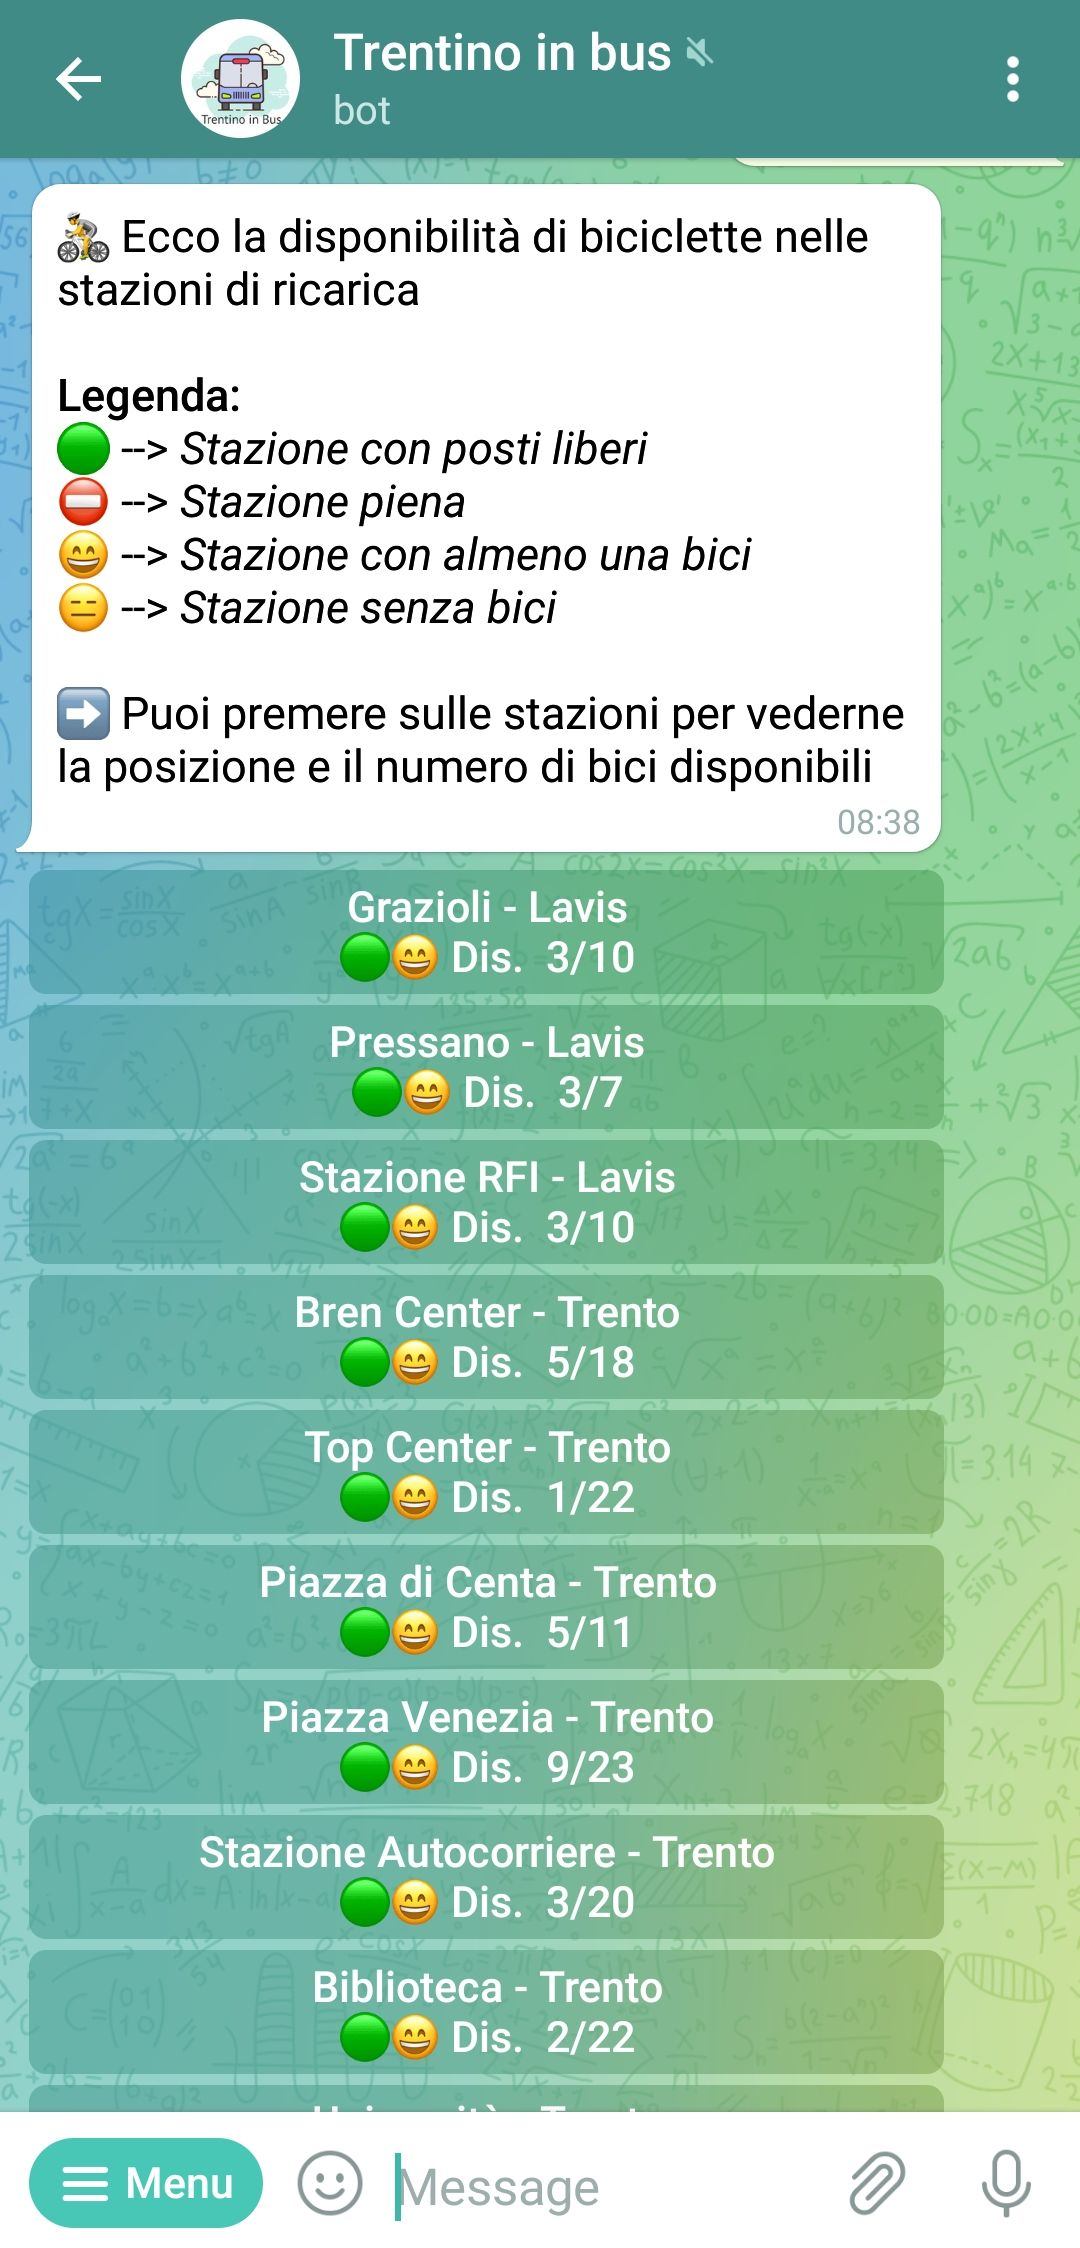
\includegraphics[width=\linewidth]{bot-stazioni-bici.jpg}}
\caption{Stazioni bici}
\label{fig:bot-stazioni-bici}
\end{subfigure}\hfil 
\begin{subfigure}{0.20\textwidth}
\frame{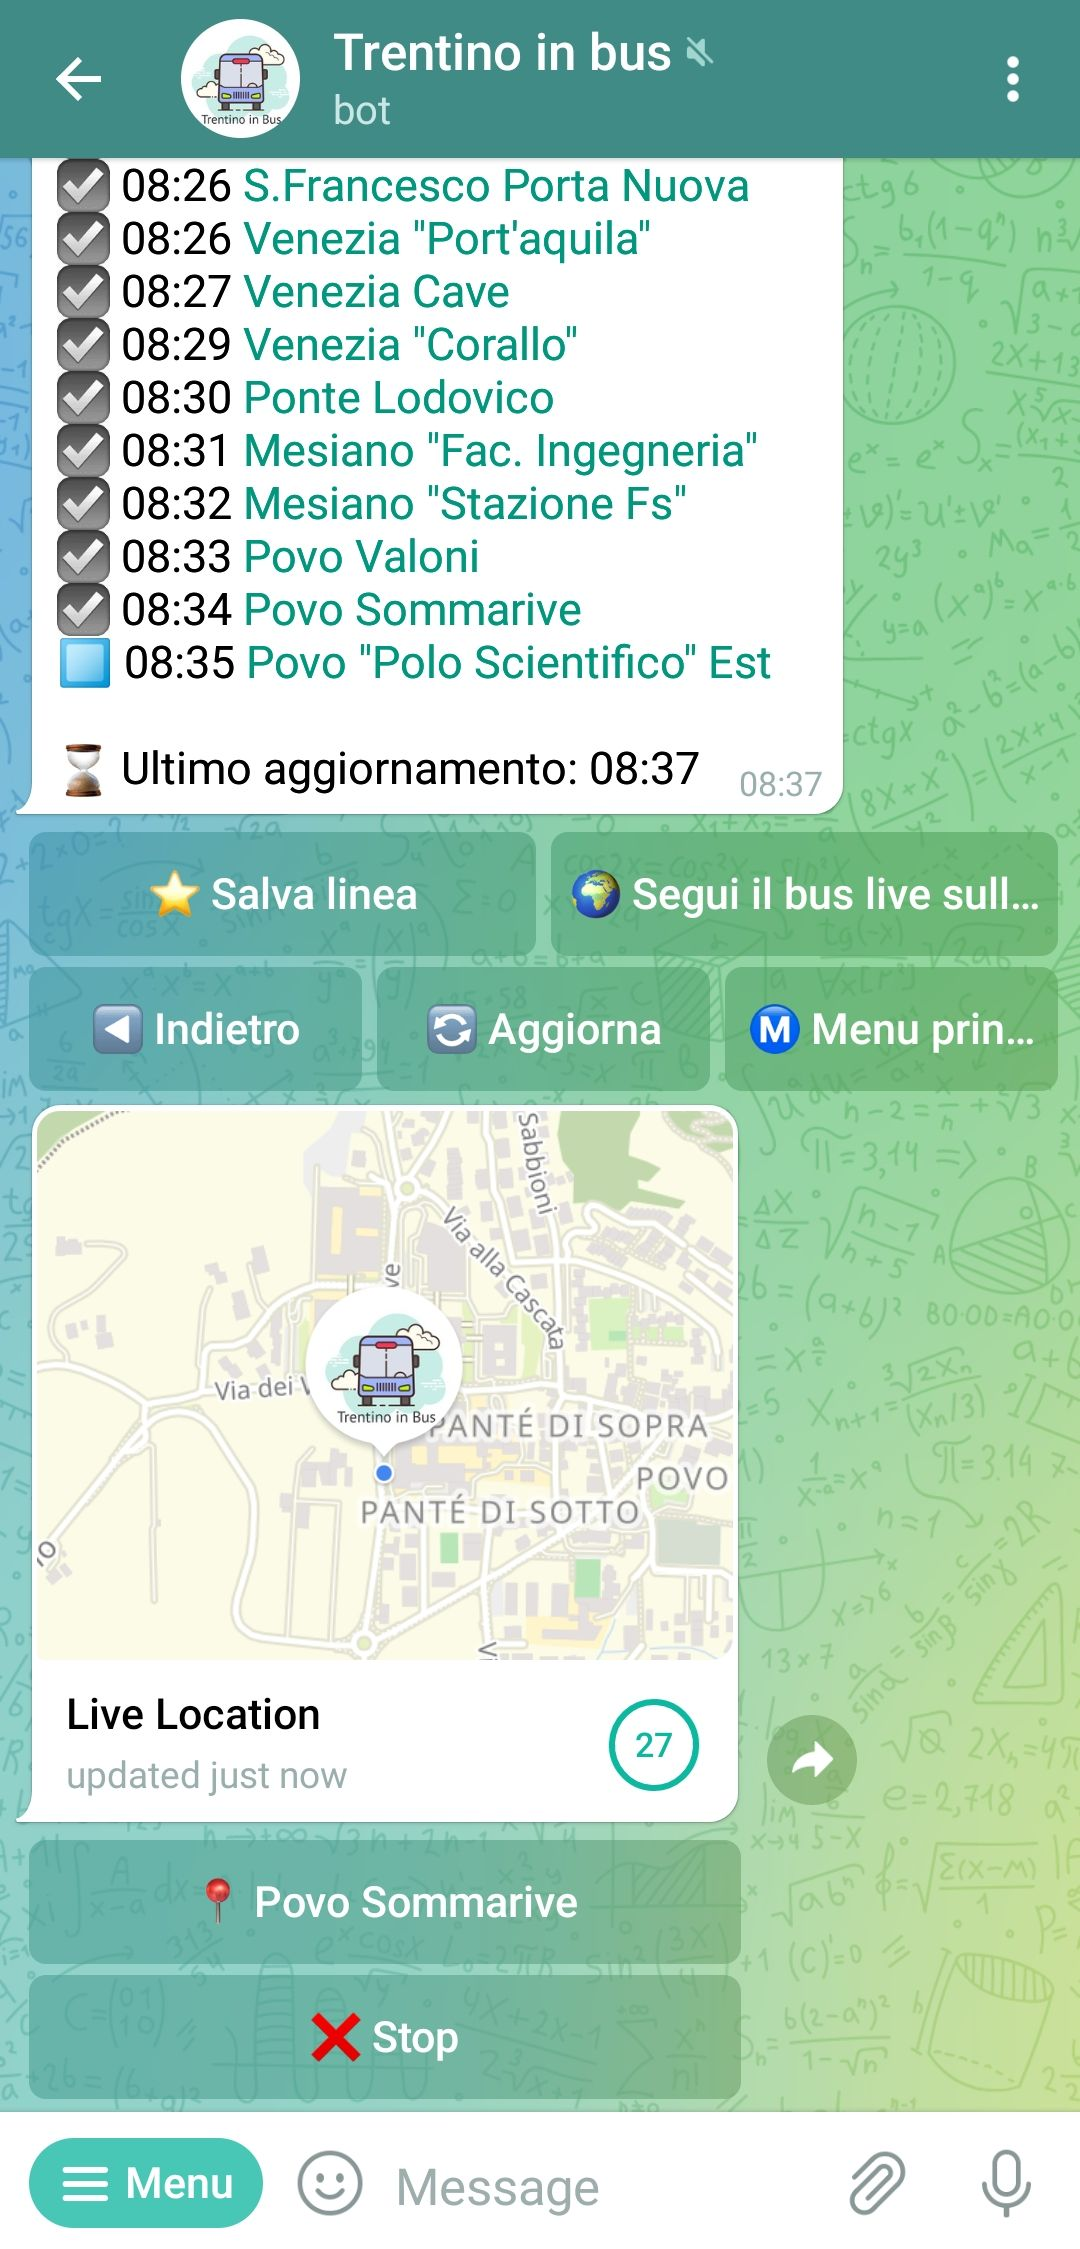
\includegraphics[width=\linewidth]{bot-posizione-autobus.jpg}}
\caption{Posizione autobus}
\label{fig:bot-posizione-autobus}
\end{subfigure}
\caption{
\label{fig:varie_funzionalita}Altre funzionalità}
\end{figure}


\subsection{Canale notizie}

\begin{wrapfigure}{r}{0.38\textwidth}
\centering
\frame{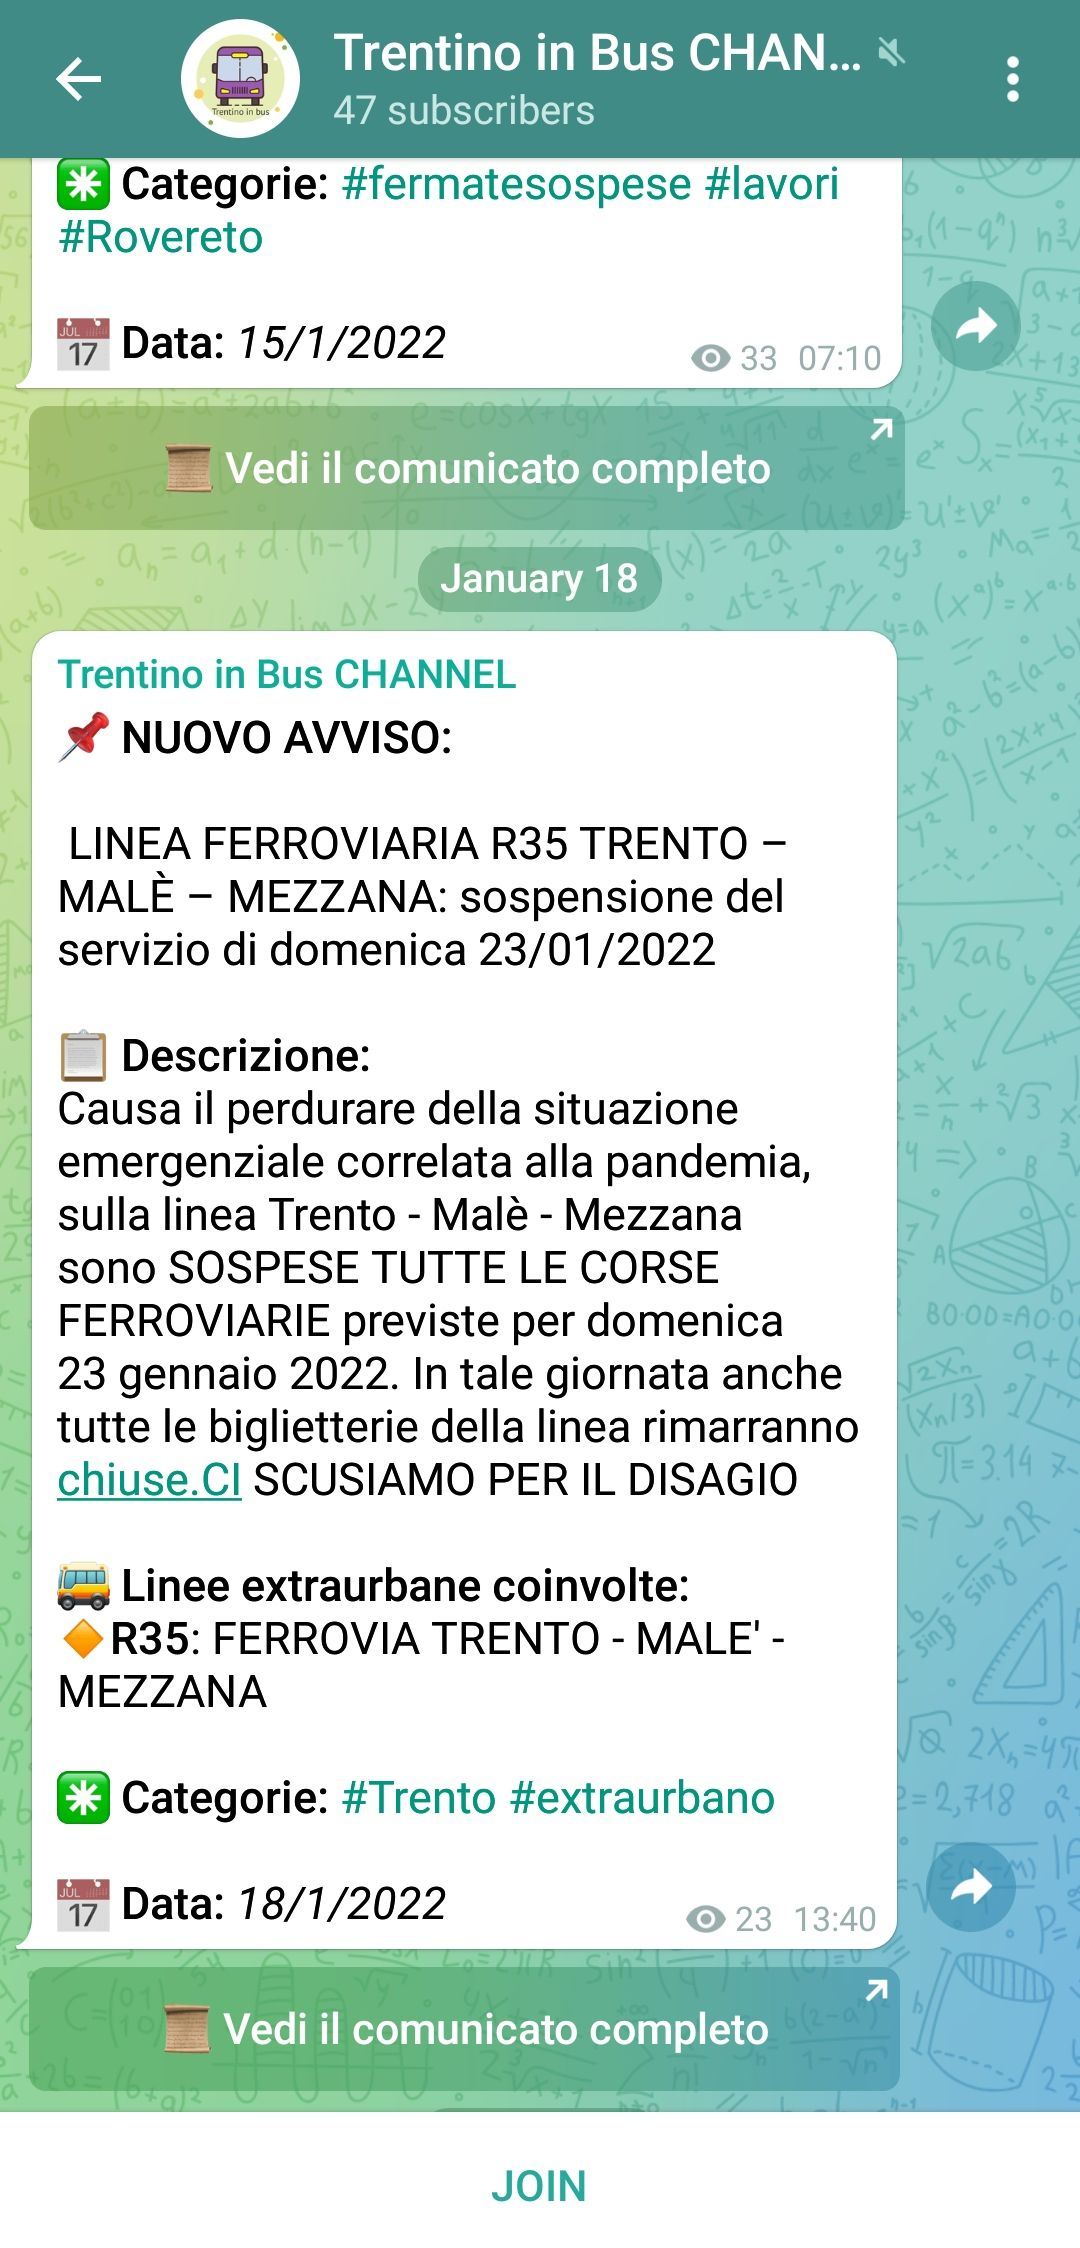
\includegraphics[scale=0.085]{bot-canale-notizie.jpg}}
\caption{Canale notizie}
\label{fig:bot-canale-notizie}
\end{wrapfigure}

Al bot principale \textit{@TrentinoInBusBot} è associato anche un canale Telegram, \textit{@TrentinoInBusChannel}, che si occupa di inviare agli iscritti aggiornamenti in tempo reale sui trasporti della Provincia di Trento. 

Questo canale è moderato automaticamente dal bot che invia al suo interno messaggi riguardanti scioperi, fermate sospese, variazioni di percorso, cambiamenti di orario, corse sospese, nuove corse e molto altro. I messaggi contengono un breve riepilogo della notizia e l'indicazione delle linee e fermate coinvolte. Anche in questo canale, come nel bot principale, i messaggi sono arricchiti dall'utilizzo di \textit{emoji} per renderli più chiari e accattivanti.

Le notizie di questo canale sono filtrabili attraverso dei tag per categoria in modo da essere facilmente ricercabili dagli utenti. Ad ogni messaggio è allegato un pulsante attraverso il quale è possibile scaricare il PDF del comunicato ufficiale di Trentino Trasporti.






      \newpage
      \chapter{Contesto smart city}
\label{cha:smartcity}

Nel seguente capitolo verrà introdotto il concetto di \textit{smart city} con una particolare approfondimento alla \textit{smart mobility}. Ho deciso di presentare questo argomento poiché il bot è considerabile un servizio interno a questo ambito. Inoltre, verranno analizzate le principali applicazioni utilizzate nelle città più smart del mondo. Successivamente farò un'analisi di scalabilità e replicabilità del mio bot cercando di capire cosa si potrebbe implementare in futuro e se è possibile estenderlo per l'utilizzo in altre zone.

Innanzitutto, per \textit{smart city} si intende una città che gestisce le risorse in modo intelligente, che mira a diventare economicamente sostenibile ed energeticamente autosufficiente, ed è attenta alla qualità della vita e ai bisogni dei propri cittadini\cite{SmarCity}.

\section{Smart mobility}
\label{sec:smart-mobility}

La \textit{Smart Mobility} è uno strumento utile ad ottenere lo sviluppo sostenibile delle città. Il termine fa riferimento a: tecnologia, infrastrutture per la mobilità (parcheggi, reti di ricarica, segnaletica, veicoli), soluzioni per la mobilità (tra cui i modelli di \textit{new mobility}) e persone. Tra i principali obiettivi da raggiungere, grazie all'introduzione di queste novità, troviamo: la riduzione del traffico e dell'inquinamento, la creazione di flussi intelligenti e senza interruzioni e il rafforzamento delle economie di scala per la promozione di una mobilità che sia accessibile a tutti. \cite{SmartMobility}\\

\noindent La\textit{ Smart mobility}, fenomeno ampio e complesso, è basato sui seguenti principi:

\begin{enumerate}
    \item  \textit{Flessibilità}: grazie alle molteplici modalità di trasporto chi si sposta ha la possibilità di scegliere quale di queste è la migliore in base al contesto;
    \item  \textit{Efficienza}: permette al viaggiatore di arrivare a destinazione con il minimo sforzo e nel più breve tempo possibile;
    \item  \textit{Integrazione}: il tragitto completo viene pianificato integrando tutti i mezzi disponibili;
    \item \textit{Tecnologie pulite}: lo spostamento dai veicoli inquinanti a quelli a zero emissioni;
    \item \textit{Sicurezza}: drastica riduzione di morti e feriti; 
    \item \textit{Accessibilità}: la \textit{smart mobility} deve poter essere accessibili a tutti, in tutte le sue forme;
    \item \textit{Benefici sociali}: la \textit{smart mobility} deve aiutare a migliorare la qualità della vita. 
\end{enumerate}

\subsection{Esempi}

\subsubsection{Smart parking}

\begin{wrapfigure}{r}{0.4\textwidth}
\centering
\frame{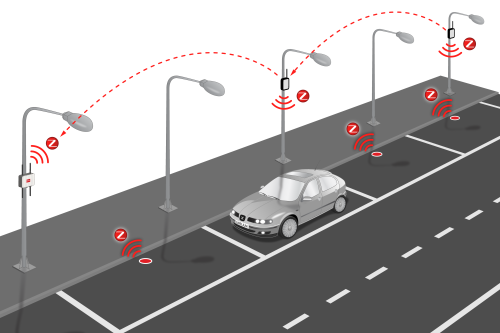
\includegraphics[scale=0.7]{smart-parking.png}}
\caption{Smart parking}
\label{fig:smart_parking}
\end{wrapfigure}

Secondo alcune statistiche, il 40\% del traffico nelle aree urbane è provocato dai guidatori che stanno cercando parcheggio, causando congestione, rumore e inquinamento. Barcellona, ad esempio, per migliorare questa situazione ha adottato la tecnologia dei parcheggi intelligenti. Nelle strade, è stato installato un sistema di sensori che comunicano ai cittadini, tramite applicazioni e dispositivi mobili, la condizione dei posti auto disponibili. Utilizzando display e \textit{embeddando} sensori nelle aree \textit{free parking}, uniti ad app che consentono la ricezione delle informazioni e la gestione dei pagamenti, Barcellona è riuscita a rendere più fluido il traffico, ridurre il tempo e il carburante richiesto, portando benefici anche all'ambiente.  

Tra i servizi di \textit{smart parking} troviamo, ad esempio, il \textit{“community-based parking”}: dei veicoli connessi tra loro con un hardware di connettività identificano, attraverso dei sensori, gli spazi disponibili mentre passano. Ciò permette agli automobilisti, in cerca di parcheggio, di beneficiare di questi dati acquisiti dalla "comunità" e di essere guidati sul posto con informazioni in tempo reale. 

\subsubsection{Semafori intelligenti}

In Olanda, sull’autostrada N205 a Noord-Holland, vicino ad Amsterdam, sono presenti dei semafori in grado di "parlare" in tempo reale, attraverso un'applicazione, con i viaggiatori. Le informazioni fornite riguardano le condizioni del traffico e permettono di dare priorità a determinati gruppi di automobilisti. Inoltre, già a partire dal 2016, sono stati installati, nella città di 's-Hertogenbosch, dei semafori smart in grado di regolare la durata del verde in base alle esigenze del traffico. Quando, ad esempio, i semafori registrano una maggiore affluenza di biciclette, automobili o mezzi di trasporto pubblico prolungano il via libera, così da non creare ingorghi. 

\subsubsection{Mobility As A Service (MaaS)}

\begin{wrapfigure}{r}{0.4\textwidth}
\centering
\frame{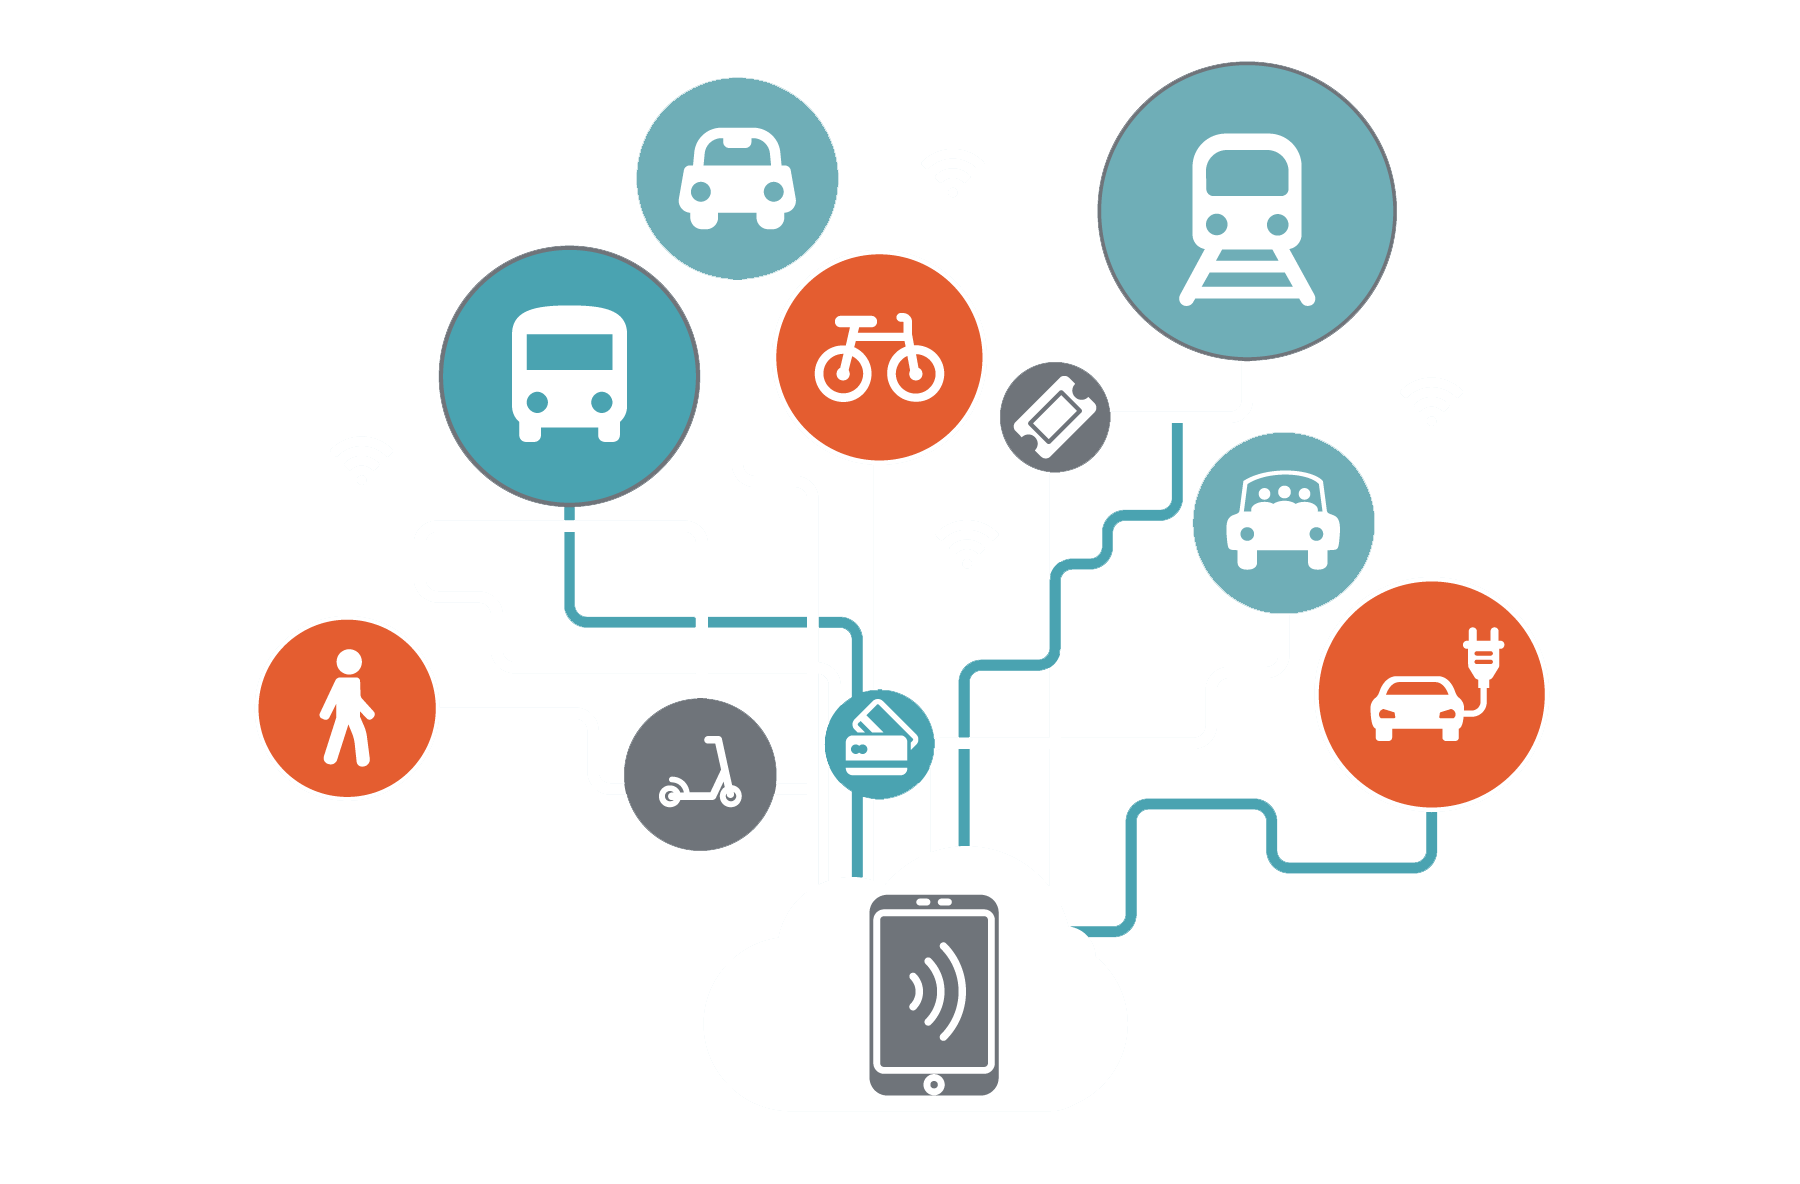
\includegraphics[scale=0.095]{maas.png}}
\caption{MaaS app}
\label{fig:maas}
\end{wrapfigure}

Il \textit{MaaS} (Mobility as a Service) rappresenta un nuovo modello di business per l'erogazione di servizi di trasporto. Come tutti i modelli \textit{"as a service"}, prevede un abbonamento mensile a regime forfait che assicura l'utilizzo personalizzato di un \textit{bundle} di trasporti pubblici e privati, che siano treni, bus, taxi, car o bike sharing, in modo illimitato con un unico abbonamento (\textit{all in one}), tendenzialmente attraverso un'app. 

L’Autorità del Trasporto regionale di Helsinki consente l’accesso ai dati relativi a percorsi, orari e costi attraverso le API aperte. L’app è inoltre integrata con i calendari degli utenti in modo che questi possano programmare in anticipo il proprio viaggio e scegliere in base a criteri come velocità, prezzo e comfort.

\section{Competitor}
\label{sec:competitor}

Dopo aver approfondito il concetto di \textit{smart mobility} è importante fare un'analisi dei potenziali servizi competitor. Questo permette di stabilire cosa manca nel mercato attuale e conoscere le preferenze degli utenti, oltre a rendere più chiaro in che direzione sarà possibile scalare il bot Telegram.

\subsection{Bot telegram}
Innanzitutto, sono partito ricercando dei bot telegram legati alla mobilità. La ricerca non è stata banale dato che non esiste un sistema centrale, come può essere ad esempio il \textit{Play Store} per le applicazioni mobile Android, che raccoglie e categorizza i bot esistenti e verifica il loro stato. Quindi, i bot sono stati ricercati tramite \textit{Google} e tramite \textit{BotsArchive}, un sito web che tramite segnalazione degli utenti o sviluppatori raccoglie i bot Telegram e permette agli utenti di votare i migliori. Sfortunatamente, molti di questi risultavano offline e non è stato quindi possibile testarli ed inserirli in questo approfondimento, sebbene sembrassero molto validi.

\subsubsection{ViaggiaTrentoBot}

\textit{ViaggiaTrentoBot} supporta la mobilità urbana sostenibile di Trento. Esso permette di consultare gli orari degli autobus urbani di Trento e dei treni delle ferrovie Brennero, Valsugana e Trento-Mezzana. Inoltre, permette di controllare in diretta i posti liberi nei parcheggi e la disponibilità di biciclette nei punti di bike sharing della città. L'interfaccia è abbastanza intuitiva ma, sfortunatamente, è limitato alla sola città di Trento e non fornisce informazioni sulla posizione dei mezzi in tempo reale.

\subsubsection{GTT Orari degli arrrivi in fermata}
Questo bot consente di conoscere gli arrivi previsti alla fermata dei tram e dei bus urbani e suburbani di Torino e di visualizzare le rivendite autorizzate di biglietti più vicine. Per le ricerche è sufficiente inserire il numero della fermata di interesse riportato sulla fermata, oppure il nome della fermata voluta; a questo punto si riceverà un messaggio con gli orari dei passaggi in tempo reale ed una mappa in cui è mostrata la posizione della fermata e la zona circostante. L'interfaccia di questo bot è confusionaria ed è difficile da utilizzare senza essere guidati.

\subsubsection{TrenItBot}

TrenItBot è un bot di Telegram che ti permette di cercare e seguire i treni italiani mostrandoti orari, ritardi, binari, fermate, cancellazioni e scioperi in tempo reale. Se si conosce il numero del treno che si vuole seguire, si può inviare il comando \textit{/segui}. Altrimenti, usando il comando \textit{/cerca} è possibile trovare una soluzione di viaggio se si conosce la stazione di origine, quella di destinazione, e l'orario (approssimato) di partenza. Il bot è molto intuitivo anche per utenti al primo utilizzo ed è, secondo me, il migliore provato di questa categoria.

\subsubsection{Altri bot}
Quasi tutti i bot Telegram legati alla mobilità di città non italiane erano offline, in particolare ho trovato dei bot per le città di Dublino e Madrid. L'unico funzionante che ho trovato è \textit{Bus Eta Bot}. Questo permette di conoscere, in tempo reale, il tempo di arrivo previsto degli autobus di Singapore e fornisce altre informazioni sull'autobus in arrivo come il tipo di autobus, l'affluenza e se è accessibile o meno in sedia a rotelle.

\begin{figure}[htb]
    \centering 
\begin{subfigure}{0.20\textwidth}
\frame{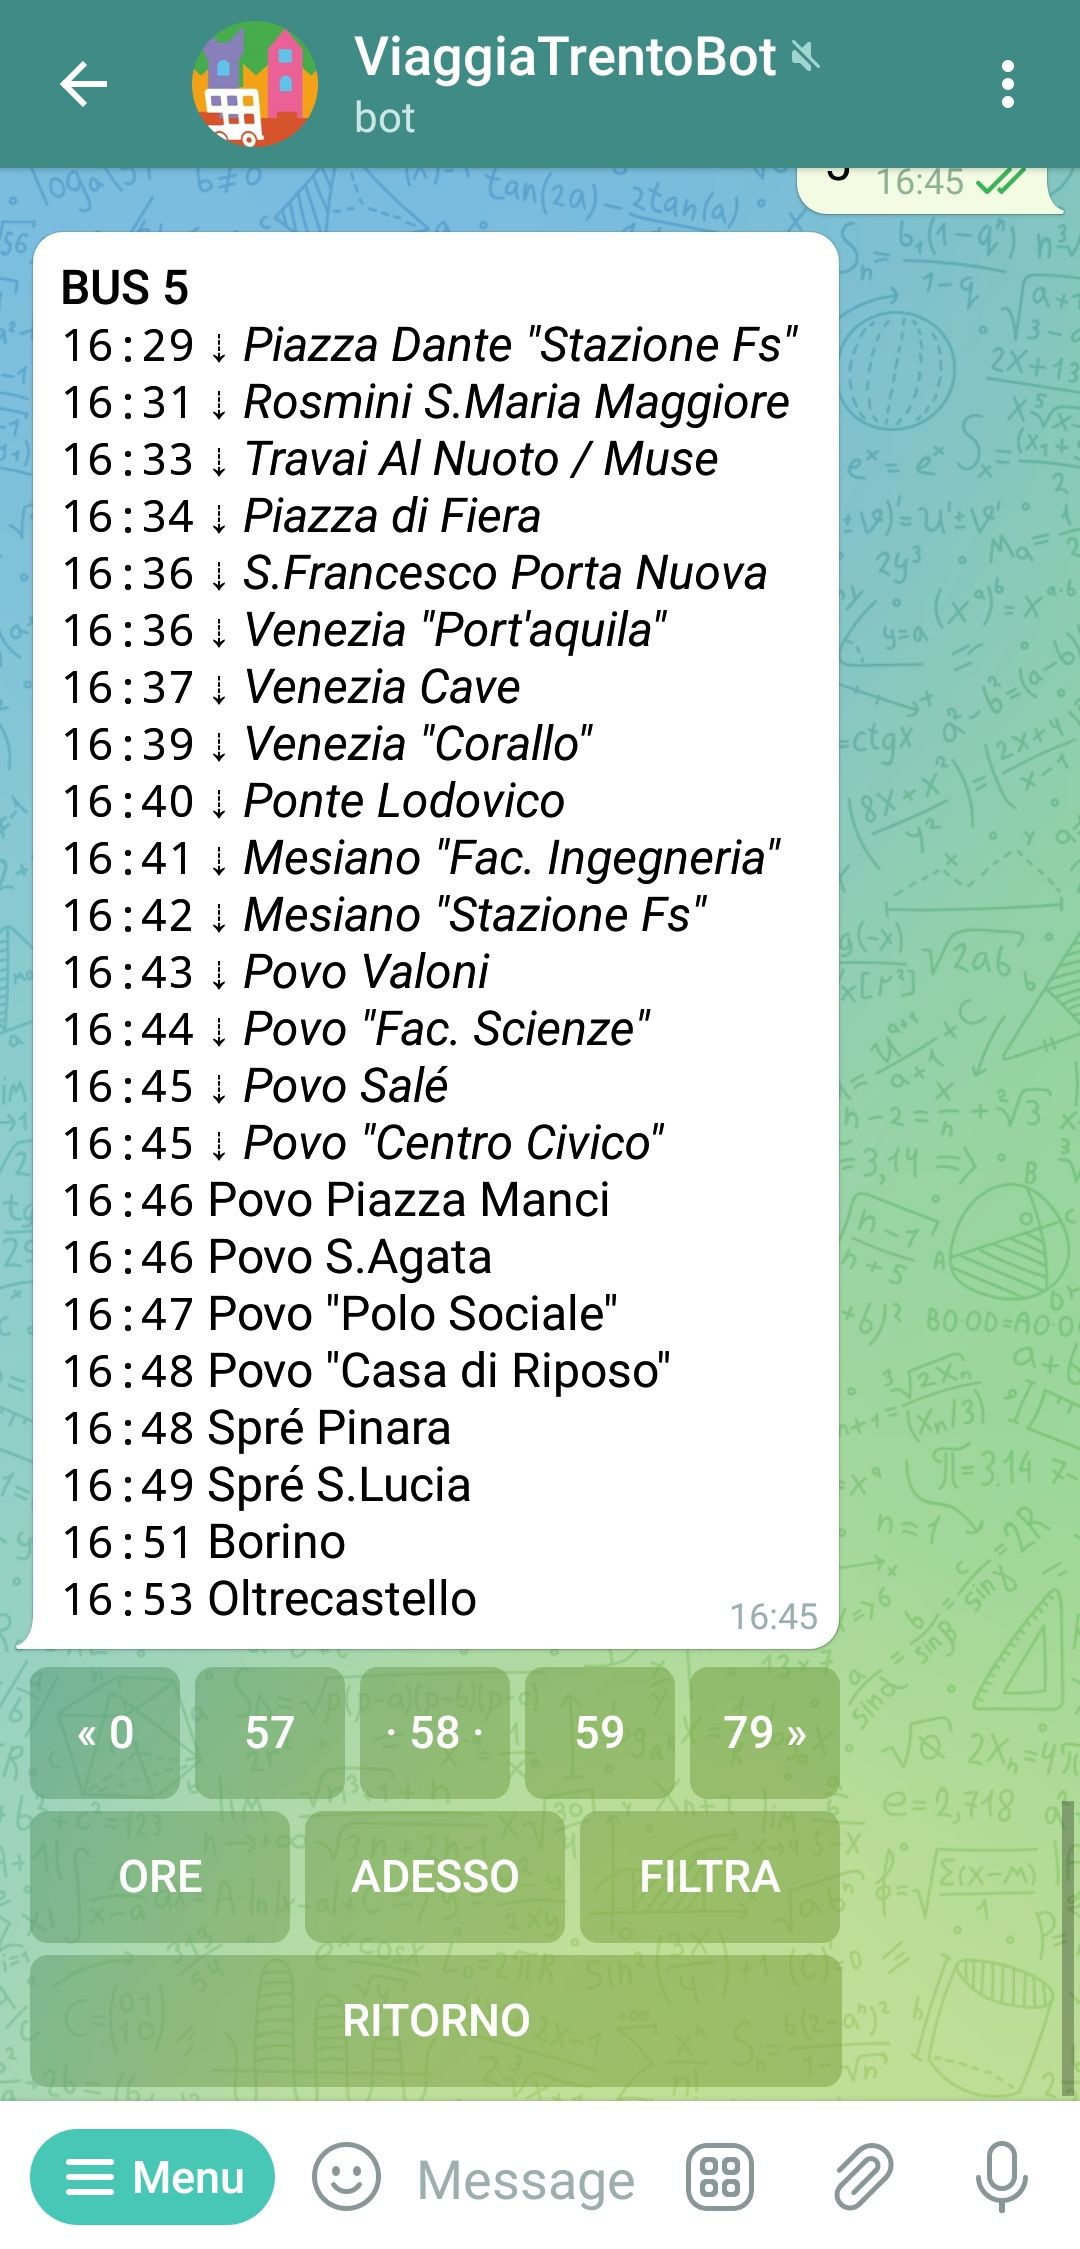
\includegraphics[width=\linewidth]{competitor_viaggiatrento.jpg}}
\caption{ViaggiaTrentoBot}
\label{fig:viaggia_trento}
\end{subfigure}\hfil
\begin{subfigure}{0.20\textwidth}
\frame{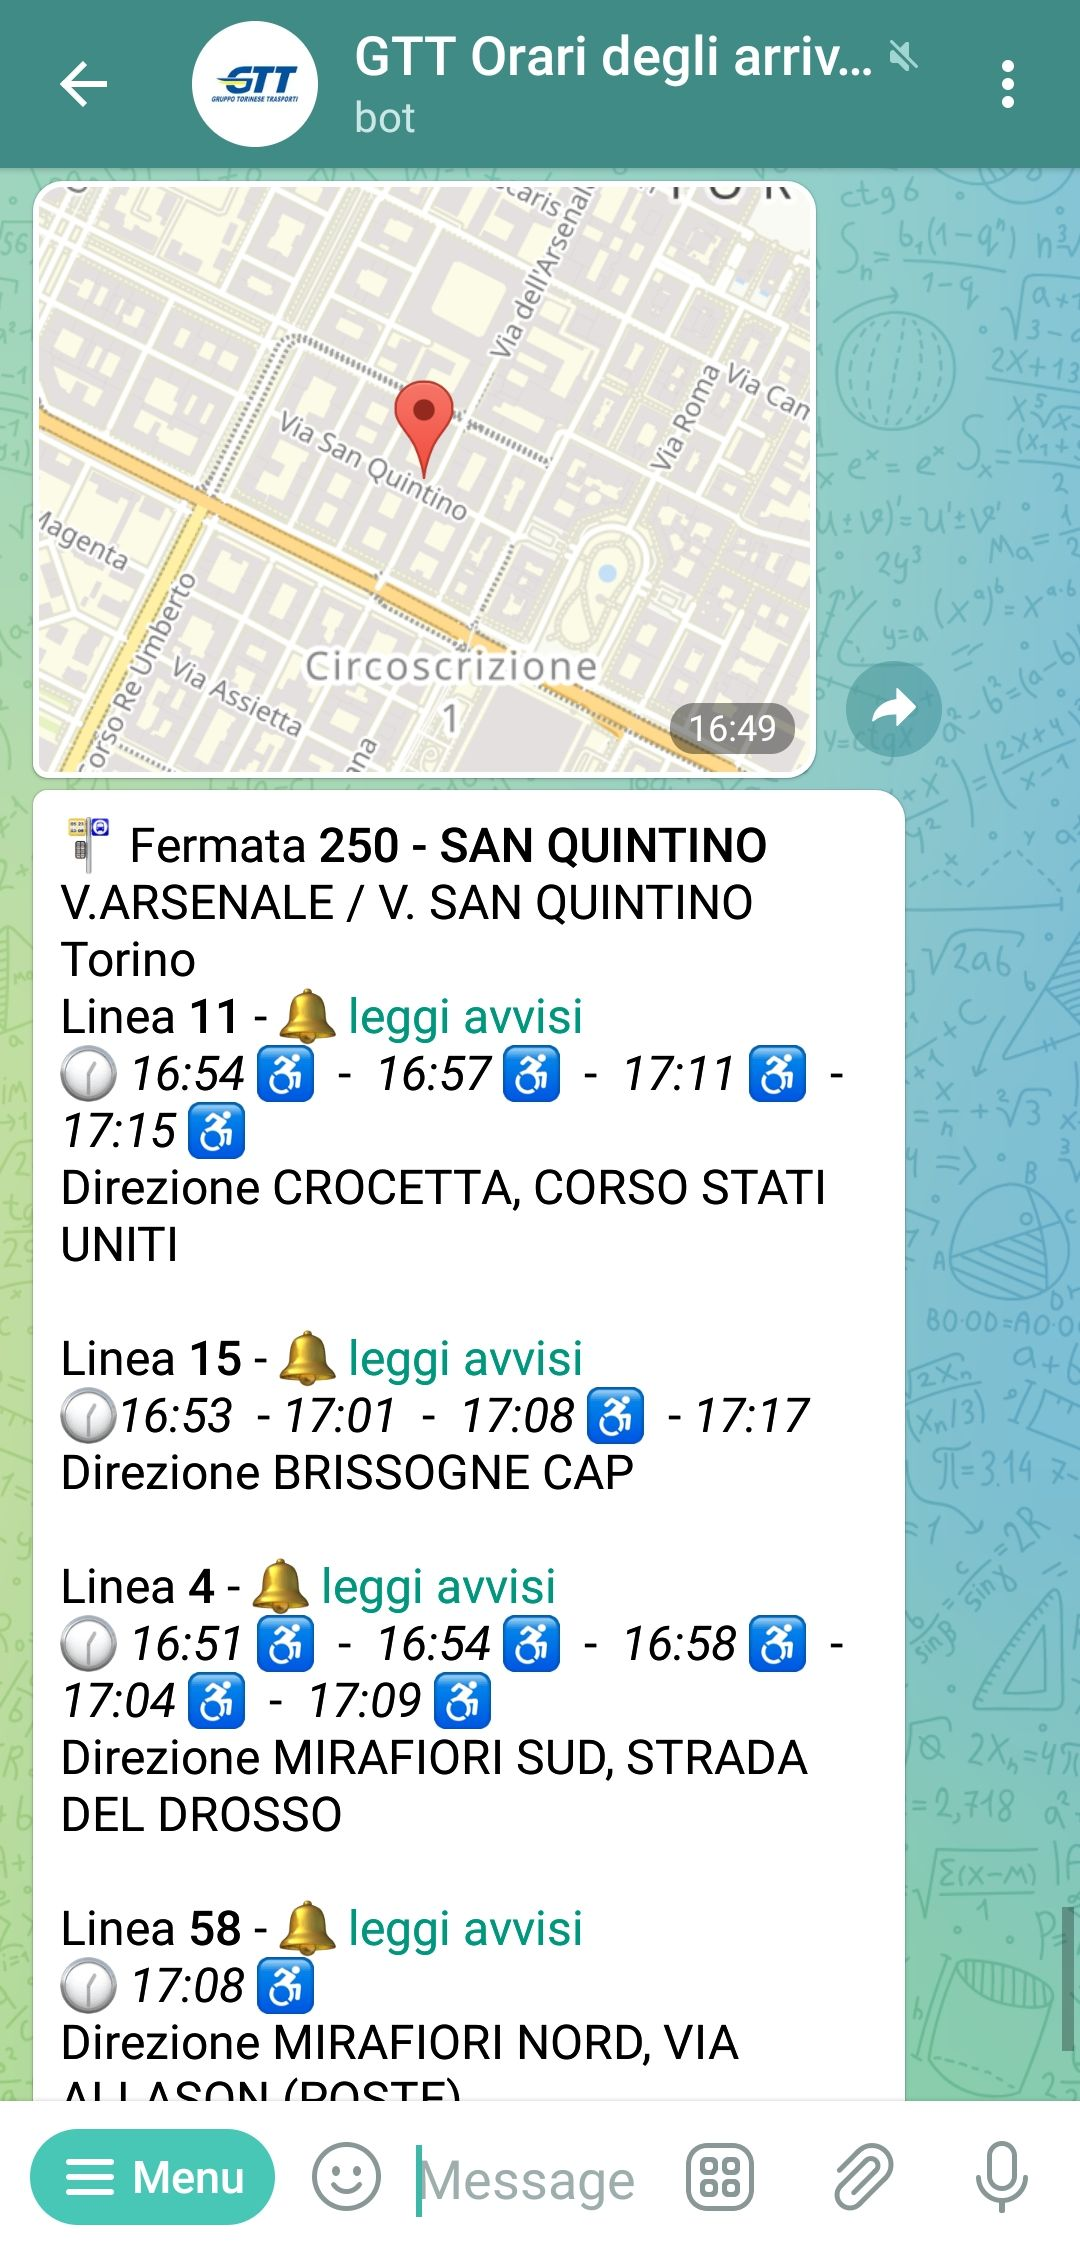
\includegraphics[width=\linewidth]{competitor_gtt.jpg}}
\caption{GTT Orari}
\label{fig:gtt_orari}
\end{subfigure}\hfil 
\begin{subfigure}{0.20\textwidth}
\frame{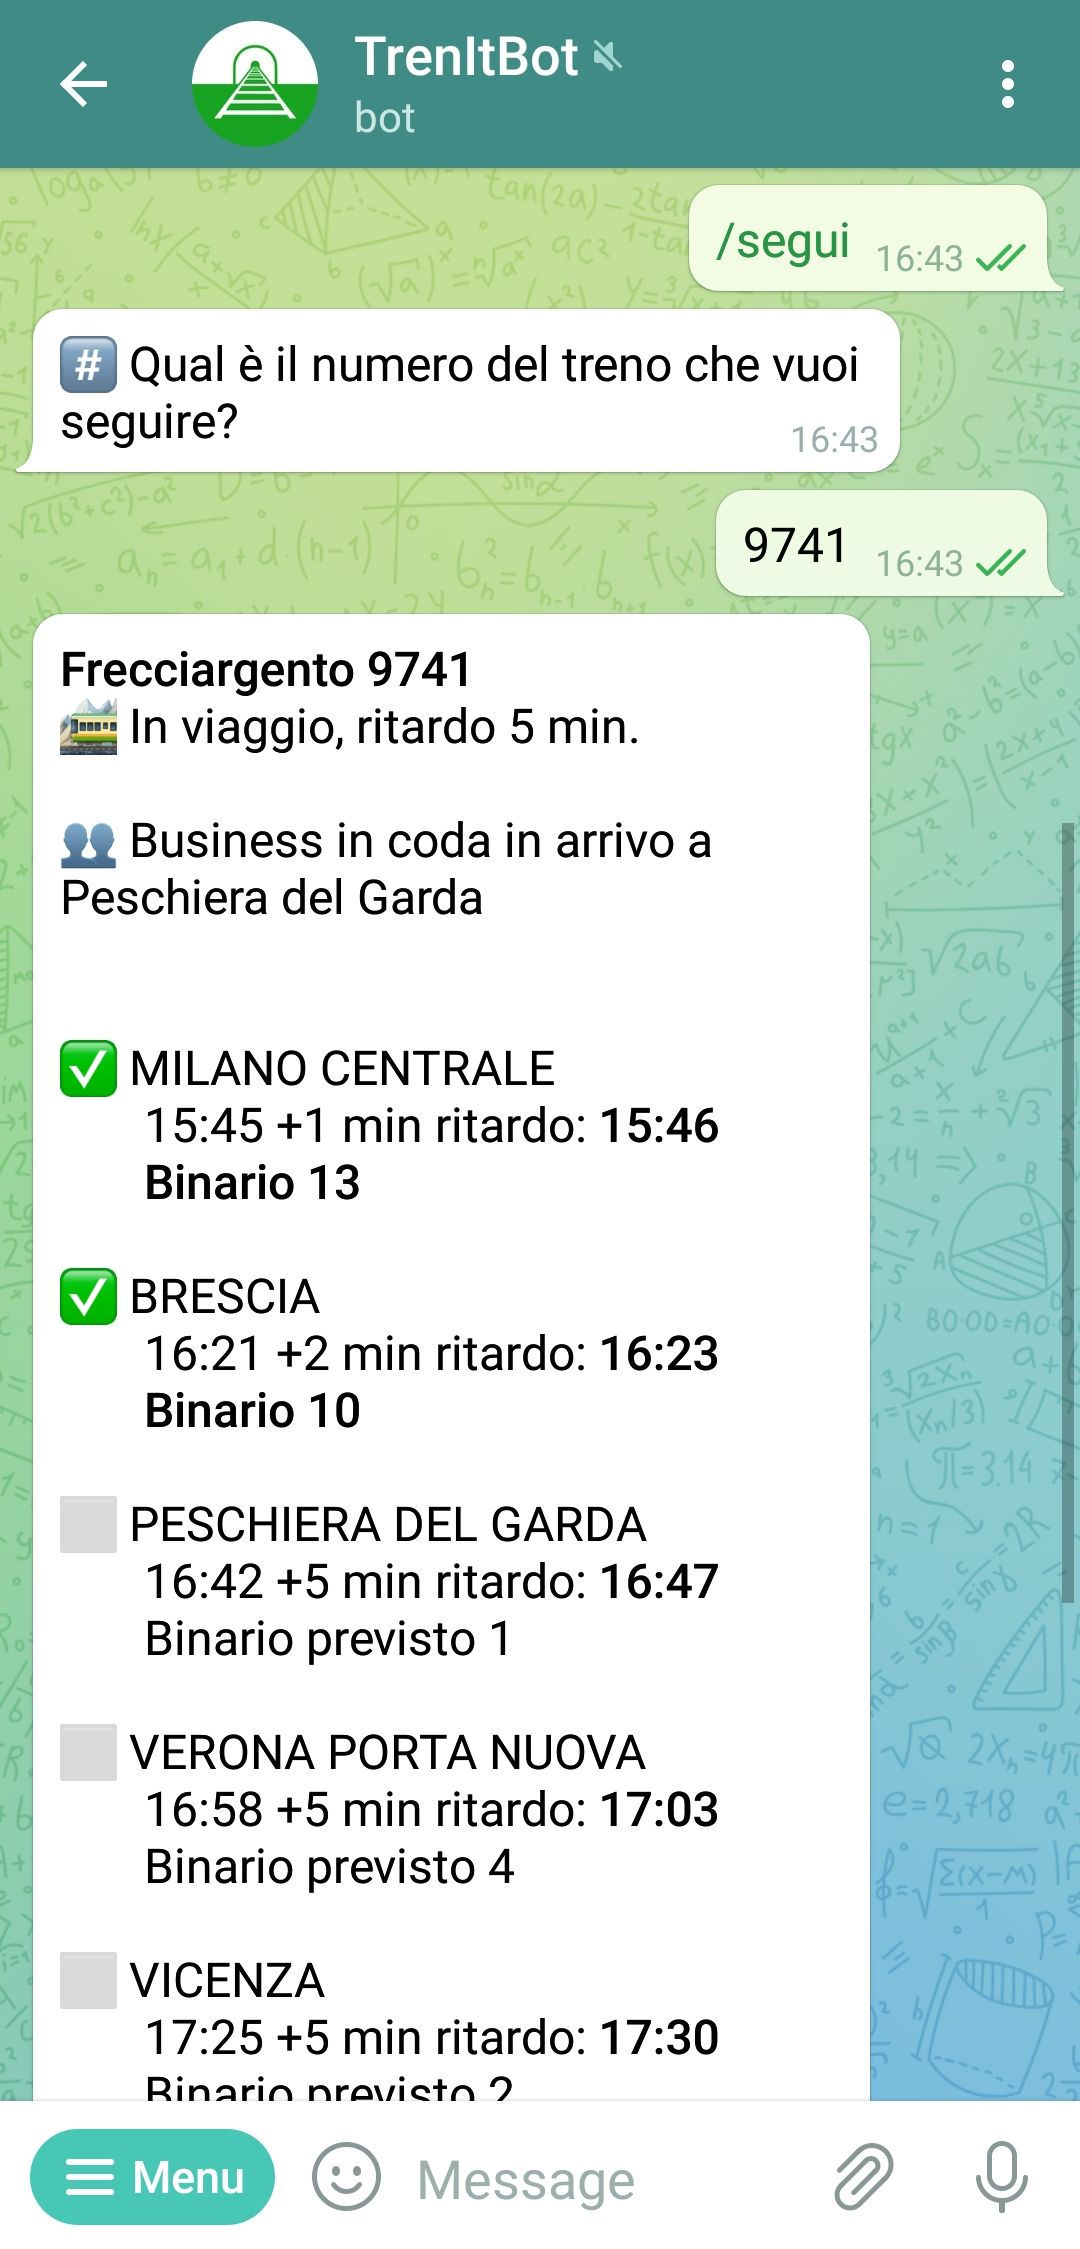
\includegraphics[width=\linewidth]{competitor_trenitbot.jpg}}
\caption{TrenItBot}
\label{fig:trenit_bot}
\end{subfigure}\hfil 
\begin{subfigure}{0.20\textwidth}
\frame{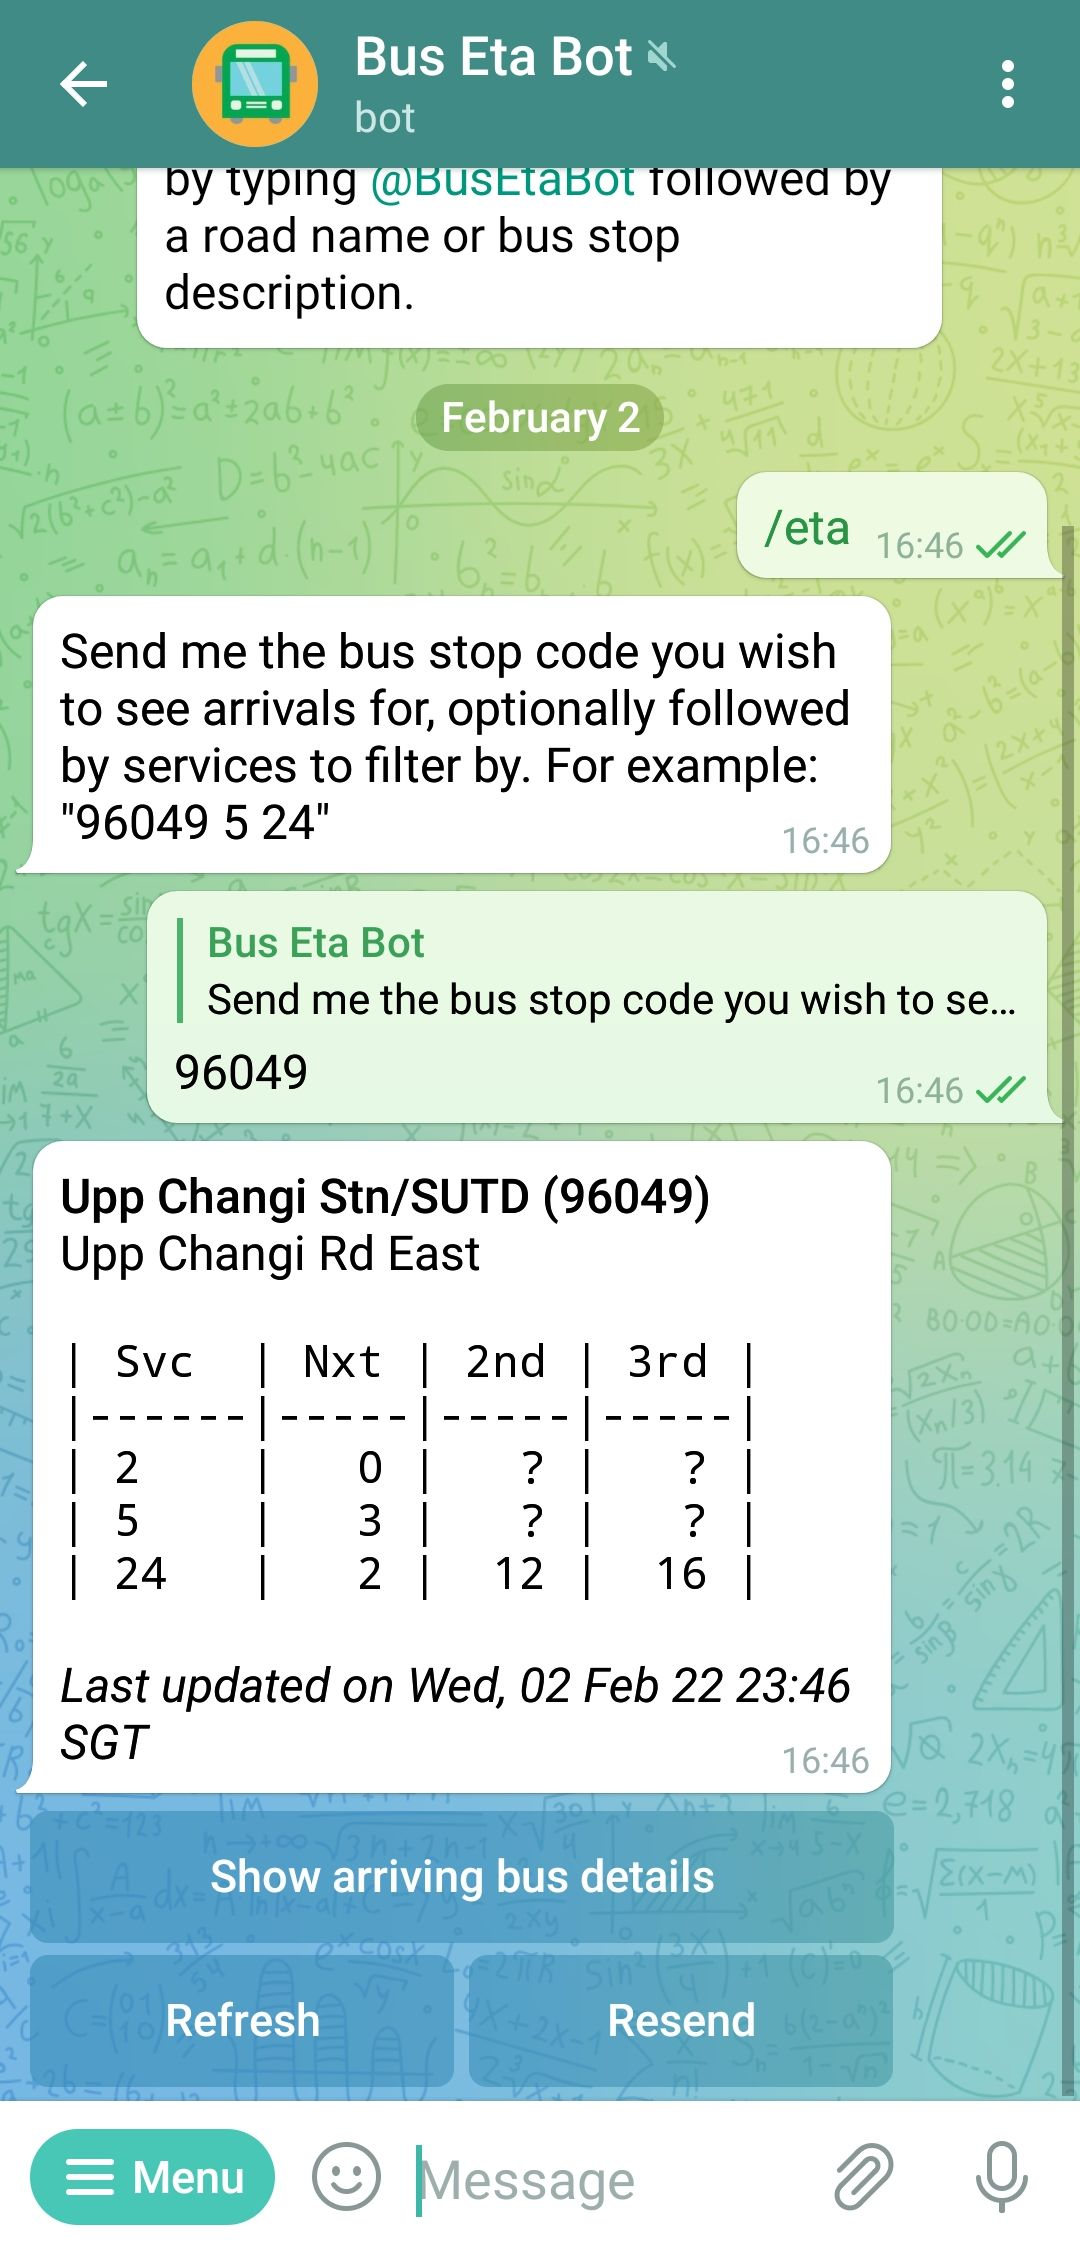
\includegraphics[width=\linewidth]{competitor_buseta.jpg}}
\caption{Bus Eta Bot}
\label{fig:bus_eta_bot}
\end{subfigure}
\caption{
\label{fig:bot_competitor}Bot telegram competitor}
\end{figure}

\subsection{Applicazioni mobile}
A differenza dei bot Telegram, non è stato difficile trovare applicazioni mobile legate alla \textit{smart mobility} operanti sia nel mondo che in Italia. Nonostante la diffusione di questi progetti a livello locale dia una grande spinta all’adozione di modelli di vita più sostenibili, sfortunatamente, non c’è ancora un servizio che possa essere utilizzato in tutta Italia, indipendentemente dalla regione e dalla città di residenza. Questo pone dei limiti, soprattutto per chi viaggia spesso all’interno dei confini nazionali. Di seguito ho deciso di riportare e descrivere brevemente tre applicazioni attualmente attive nel settore della \textit{smart mobility} che offrono dei servizi originali.

\subsubsection{Moovit}

\begin{wrapfigure}{r}{0.50\textwidth}
\centering
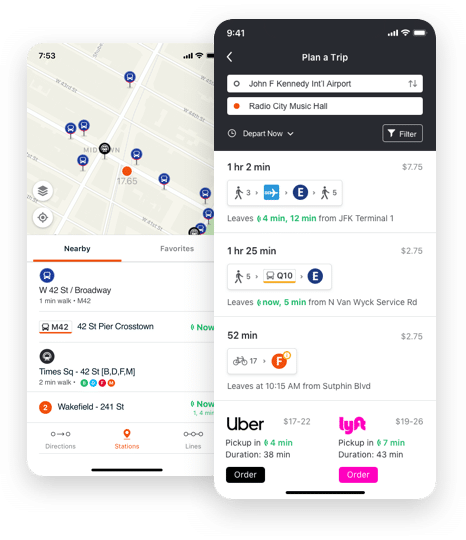
\includegraphics[scale=0.45]{app_moovit.png}
\caption{App Moovit}
\label{fig:app_moovit}
\end{wrapfigure}

 Questa azienda, leader mondiale di soluzioni di \textit{MaaS} (Mobility as a Service) e di \textit{journey planning}, ora proprietà di \textit{Intel}, nasce come start-up israeliana. L'app consente di pianificare e pagare un percorso, scegliendo il tragitto e il mezzo più conveniente, tutto attraverso lo smartphone. Ciò è reso possibile combinando dati ufficiali a \textit{crowdsourced data} (dati ottenuti dagli utenti attraverso la rete), questo permette di fornire informazioni in tempo reale sui servizi di trasporto pubblico. A questo si aggiungono i dati su taxi, Uber, Lyft, biciclette, monopattini, scooter e ciclomotori, car sharing e molto altro. Inoltre, l'app, attraverso notifiche push, informa gli utenti su variazioni al servizio di trasporto pubblico o allerte meteo. 
 Attualmente è disponibile in Italia solo nelle grandi città. Essa è in continuo aggiornamento, infatti, tra gli ultimi aggiornamenti pubblicati troviamo, ad esempio, i dati sull'affluenza dei singoli bus in tempo reale, tramite la segnalazione degli utenti. 
 Esistono molte app simili come ad esempio Transit e Citymapper, ma Moovit è la più completa nel suo genere.

\subsubsection{EasyPark}

\begin{wrapfigure}{r}{0.55\textwidth}
    \centering 
\begin{subfigure}{0.23\textwidth}
\centering
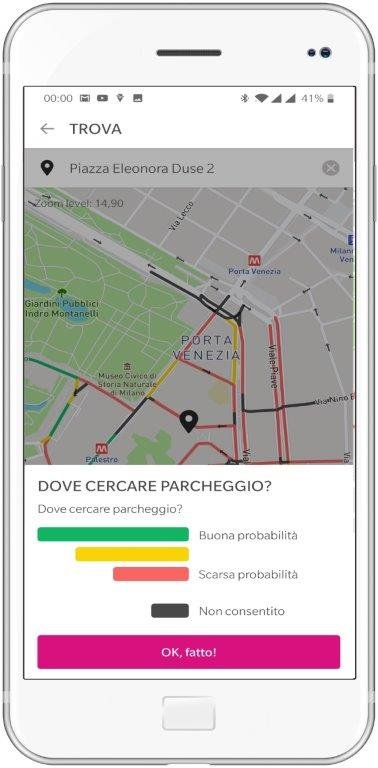
\includegraphics[scale=0.55]{app_easypark.jpg}
\caption{Ricerca parcheggio}
\label{fig:app_easypark_1}
\end{subfigure}\hfil
\begin{subfigure}{0.23\textwidth}
\centering
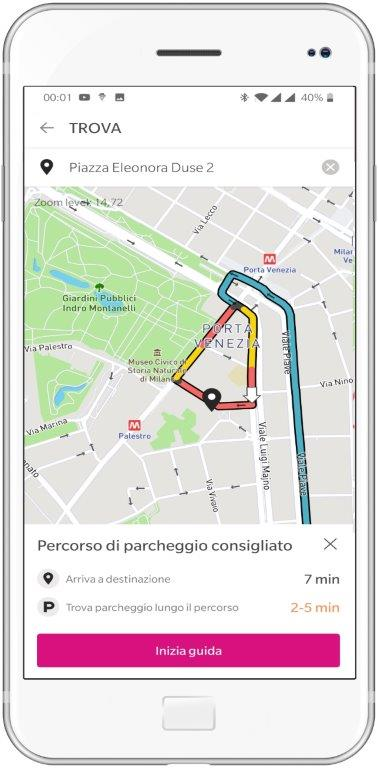
\includegraphics[scale=0.55]{app_easypark_2.jpg}
\caption{Percorso consigliato}
\label{fig:app_easypark_2}
\end{subfigure}
\caption{
\label{fig:app_easypark}App EasyPark}
\end{wrapfigure}

Questa app offre una visione completa delle diverse soluzioni di sosta, di breve o lunga durata, comprese di prezzi e distanza dalla destinazione prescelta. All'interno dell'app troviamo diversi servizi:
\begin{itemize}
    \item \textit{parking planner}, che permette la prenotazione del parcheggio in anticipo;
    \item \textit{parking guidance}, che aiuta a trovare posti auto disponibili nella città;
    \item  \textit{find park}, strumento che fornisce il percorso ottimale per trovare parcheggi su strada o garage disponibili vicino ad un luogo d'interesse, unito ad una mappa in cui i colori delle vie chiariscono la probabilità di trovare parcheggio (Vedi figura \ref{fig:app_easypark}\subref{fig:app_easypark_1}).
\end{itemize} 


\noindent Inoltre, è possibile gestire la sessione di sosta in base alle proprie necessità, pagando, attraverso diverse modalità, solo il tempo d'uso effettivo senza rischio di multe o bisogno di parchimetri. 

\subsubsection{BusLive}

Questa app, meno conosciuta delle precedenti, permette di visualizzare la posizione GPS dei mezzi di trasporto pubblico. Questo permette di pianificare i trasferimenti tenendo conto della reale situazione del traffico e scegliendo il veicolo che permette di arrivare nel luogo selezionato nel minor tempo possibile.
Nonostante l'idea di base sia molto buona, l'interfaccia utente e il design potrebbero essere maggiormente curati. 
Questo servizio è disponibile solo in due città italiane, Roma e Torino, e in alcune città della Polonia.

\section{Sviluppi futuri @TrentinoInBusBot}
\label{sec:sviluppi_futuri}

\begin{wrapfigure}{r}{0.38\textwidth}
\centering

\includegraphics[scale=0.2]{TrentinoInBus.jpg}
\caption{Logo TrentinoInBus}
\label{fig:trentino_in_bus}
\end{wrapfigure}

Dopo aver approfondito il concetto di \textit{Smart Mobility} e analizzato alcuni dei migliori servizi sul mercato, ho eseguito un brainstorming su come poter migliorare ed espandere il bot. 

Sicuramente sarebbe interessante orientarsi verso una soluzione \textit{MaaS}, aggiungendo informazioni sui servizi in sharing e di micro-mobilità, e permettendo agli utenti di organizzare i propri spostamenti fornendo varie opzioni. Se ci si orienta verso questa soluzione sarebbe poi necessario implementare un sistema di pagamento direttamente nel bot. Fortunatamente Telegram, tramite le sue \textit{Bot Payments API}, mette a disposizione delle API per ricevere pagamenti per beni e servizi dagli utenti. Telegram e lo sviluppatore del bot non processano nessun pagamento e non accedono a nessuna informazione sensibile, ma fanno affidamento ai più famosi provider di pagamento come \textit{Stripe}.

La funzionalità di monitoraggio dei parcheggi si potrebbe anch'essa migliorare aggiungendo la possibilità di gestire e pagare la sosta direttamente dal bot e permettendo di trovare i parcheggi ottimali in base alla propria destinazione.

\subsection{Scalabilità, replicabilità, problemi e limitazioni}
\label{sec:scalabilita}
Dal punto di vista tecnico, il bot, essendo stato sviluppato utilizzando tecnologie fortemente scalabili, non presenterà alcun problema nel caso di un incremento delle funzionalità o degli utenti. Infatti, \textit{NodeJs} fornisce meccanismi di \textit{Load Balancing} e MongoDB permette di essere scalabile sia orizzontalmente, attraverso lo \textit{sharding}, che verticalmente, aggiungendo più CPU e RAM.


Il bot Telegram  potrebbe potenzialmente essere replicato ed utilizzato in ogni luogo del mondo facendo dei piccoli adattamenti e integrando le API esterne necessarie al suo funzionamento.


I problemi principali, al momento, sono connessi alla ricerca e integrazione di API pubbliche. Risulta necessario trovare delle API che permettano il supporto a più zone, quindi non solo in Trentino, e che forniscano la possibilità di integrare i pagamenti per l'acquisto di biglietti o delle soste. Fortunatamente, le API di \textit{ViaggiaTreno} utilizzate al momento nel bot, in riferimento alle informazioni sulle ferrovie, possono essere estese all'utilizzo sull'intero territorio nazionale. 

Visto il progetto di espandere il servizio, telegram, e in particolare le funzionalità offerte dai bot, potrebbero risultare limitanti andando a rendere anche più difficile l'utilizzo da parte dell'utente. Inoltre, se l'espansione riguarderà i territori coperti dal bot potrebbe risultare utile creare una serie di bot, uno per zona, con tutte le funzionalità. Questo permetterà di mantenere un'interfaccia chiara e non appesantita da troppe azioni per l'utente. 

Infine, il nome del bot, \textit{@TrentinoInBusBot}, risulta essere riduttivo e poco rappresentativo rispetto alle tante funzionalità già presenti. Potrebbe quindi essere utile rinominarlo con un nome più emblematico rispetto alle tante possibilità offerte. 



      \newpage
      \chapter{Conclusioni}
\label{cha:conclusioni}

In quest'ultimo capitolo commenterò gli obiettivi raggiunti e le funzionalità implementate. Parlerò del percorso di formazione che mi ha aiutato nella progettazione e creazione del bot, dello stato attuale del lavoro e, infine, alcune considerazioni soggettive. 

\section{Raggiungimento degli obiettivi}

Gli obiettivi prefissati per questo progetto sono stati raggiunti. Tutte le fasi necessarie alla realizzazione del bot sono state eseguite. In particolare, sono partito da una prima fase di analisi dei requisiti, per poi passare alla progettazione tecnica dei vari aspetti del bot e, infine, allo sviluppo vero e proprio. 

\subsection{Funzionalità del bot}

Come descritto nel capitolo 1, le funzionalità sviluppate sono: 
\begin{itemize}
\item consultare gli orari di autobus urbani e extraurbani;
\item consultare gli orari delle ferrovie Brennero, Valsugana e Trento-Mezzana;
\item visualizzare su una mappa dove si trova un autobus in tempo reale e avere la possibilità di seguirlo durante il suo percorso;
\item visualizzare il ritardo e l'ultima posizione conosciuta dei mezzi;
\item visualizzare il numero di posti liberi nei parcheggi dei comuni di Trento e Rovereto;
\item sapere la disponibilità di bici elettriche presenti nelle stazioni di ricarica;
\item salvare le fermate e linee preferite per una consultazione di orari e ritardi molto più veloce;
\item rimanere informati su eventuali scioperi, variazioni di percorso, fermate sospese.
\end{itemize}

\subsection{Stato attuale del lavoro e sviluppi futuri}

Al momento attuale, il bot risulta funzionante. Dalla sua pubblicazione è stato utilizzato da circa 500 utenti. 

In seguito all'approfondimento dei concetti di \textit{smart city} e \textit{smart mobility} e all'analisi di alcune applicazioni facenti parte di questi ambiti, risulta chiara la direzione verso cui evolvere il bot. In particolare, i nuovi obiettivi fissati riguardano: 
\begin{itemize}
    \item una soluzione \textit{MaaS}; 
    \item i pagamenti direttamente dal bot; 
    \item il miglioramento del monitoraggio dei parcheggi; 
    \item l'espansione del bot ad altri territori, nazionali e non. 
\end{itemize}

\section{Formazione}

Per la creazione di questo bot, lo studio delle tecnologie è stato individuale. Per la fase di analisi alcuni corsi universitari, come \textit{Ingegneria del software 1 e 2} e \textit{Human-Computer Interaction}, sono risultati fondamentali per la buona riuscita. 
Grazie all'esperienza di tirocinio formativo,  presso l'azienda \textit{Zupit}, dove ho potuto approfondire varie caratteristiche dello sviluppo web, è stato più semplice e veloce imparare nuovi linguaggi e tecnologie.

\section{Conclusioni soggettive}

Il lavoro di progettazione e implementazione mi hanno dato l'opportunità di migliorare ulteriormente la preparazione offerta dal corso di studi. Lo sviluppo di un progetto pratico sarà sicuramente utile ai fini dei futuri impegni lavorativi e come aggiunta al proprio portfolio personale. 

Grazie all'esperienza di tirocinio, ho potuto seguire per intero il processo di realizzazione di alcuni progetti, questo mi ha aiutato a migliorare la gestione delle possibili problematiche legate a ciascuna fase del mio progetto, con maggiore attenzione e prontezza. 
      %\input{capitolo4}
      
      
    \endgroup


    % bibliografia in formato bibtex
    %
    % aggiunta del capitolo nell'indice
    \addcontentsline{toc}{chapter}{Bibliografia}
    % stile con ordinamento alfabetico in funzione degli autori
    \bibliographystyle{plain}
    \bibliography{biblio}
    
%%%%%%%%%%%%%%%%%%%%%%%%%%%%%%%%%%%%%%%%%%%%%%%%%%%%%%%%%%%%%%%%%%%%%%%%%%
%%%%%%%%%%%%%%%%%%%%%%%%%%%%%%%%%%%%%%%%%%%%%%%%%%%%%%%%%%%%%%%%%%%%%%%%%%
%% Nota
%%%%%%%%%%%%%%%%%%%%%%%%%%%%%%%%%%%%%%%%%%%%%%%%%%%%%%%%%%%%%%%%%%%%%%%%%%
%% Nella bibliografia devono essere riportati tutte le fonti consultate 
%% per lo svolgimento della tesi. La bibliografia deve essere redatta 
%% in ordine alfabetico sul cognome del primo autore. 
%% 
%% La forma della citazione bibliografica va inserita secondo la fonte utilizzata:
%% 
%% LIBRI
%% Cognome e iniziale del nome autore/autori, la data di edizione, titolo, casa editrice, eventuale numero dell’edizione. 
%% 
%% ARTICOLI DI RIVISTA
%% Cognome e iniziale del nome autore/autori, titolo articolo, titolo rivista, volume, numero, numero di pagine.
%% 
%% ARTICOLI DI CONFERENZA
%% Cognome e iniziale del nome autore/autori (anno), titolo articolo, titolo conferenza, luogo della conferenza (città e paese), date della conferenza, numero di pagine. 
%% 
%% SITOGRAFIA
%% La sitografia contiene un elenco di indirizzi Web consultati e disposti in ordine alfabetico. 
%% E’ necessario:
%%   Copiare la URL (l’indirizzo web) specifica della pagina consultata
%%   Se disponibile, indicare il cognome e nome dell’autore, il titolo ed eventuale sottotitolo del testo
%%   Se disponibile, inserire la data di ultima consultazione della risorsa (gg/mm/aaaa).    
%%%%%%%%%%%%%%%%%%%%%%%%%%%%%%%%%%%%%%%%%%%%%%%%%%%%%%%%%%%%%%%%%%%%%%%%%%
%%%%%%%%%%%%%%%%%%%%%%%%%%%%%%%%%%%%%%%%%%%%%%%%%%%%%%%%%%%%%%%%%%%%%%%%%%
    

    \titleformat{\chapter}
        {\normalfont\Huge\bfseries}{Allegato \thechapter}{1em}{}
    % sezione Allegati - opzionale
    \appendix

\end{document}
